\chapter{The radial magnetic field}\label{chap:4}

The E989 main magnet is designed to produce a 1.45 T vertical dipole magnetic field which is precisely measured by use of a suite of NMR probes, as described in Chapter \ref{chap:3} Section \ref{sec:Field}. Components of the field in the radial, $B_{x}$ or $B_{r}$, and longitudinal, $B_{z}$, directions can make ppm-level contributions to the total field, which are not usually measured at E989. In the context of the muon EDM search described in this thesis, the radial magnetic field component, hereafter referred to as `the radial field', can tilt the muon spin precession plane in a manner consistent with a non-vanishing muon EDM; which could obfuscate a genuine signal. This makes the radial field a potentially limiting source of systematic uncertainty in the search for $d_{\mu}$, which must be precisely characterised. In this chapter, the development and execution of a novel technique for measuring the radial field to a precision of $<1$ ppm will be described, and the results of measurements performed in Run-4 will be shown. Additionally, a method for extrapolating the results of these measurements as a means of estimating the average radial field, $\langle B_{r} \rangle$, in any E989 dataset, including Run-1, will be presented.

\section{The significance of the radial field}

The existence of non-zero field components besides the vertical has significance to both the measurement of $a_{\mu}$ and the search for a muon EDM. In the case of $a_{\mu}$, $B_{x}$ ($B_{r}$) and $B_{z}$ can modify the anomalous precession frequency, $\omega_{a}$, by 
%
\begin{equation}
  \vec{\omega}_{a}=a_{\mu}\frac{e}{m_{\mu}}\vec{B}=a_{\mu}\frac{e}{m_{\mu}}(B_{x}\hat{x}+B_{y}\hat{y}+B_{z}\hat{z}).
  \label{eqn:omegaa_with_field_components}
\end{equation}
%
In the case the EDM, both $B_{r}$ and $B_{z}$ result in a tilted muon spin precession plane, with $B_{z}$ causing a longitudinal tilt and $B_{r}$ a radial tilt, as illustrated in Figure \ref{fig:Tilt2}. Both manifest as an oscillation in the average vertical muon decay angle, $\langle\theta_{y}\rangle$. In the context of a vertical decay angle based muon EDM search, such as described Chapter \ref{chap:2} Section \ref{subsec:VerticalAngleBasedSearch}, the oscillation produced by $B_{z}$ is in-phase with $\omega_{a}$ and is therefore absorbed by the cosine term in the vertical angle fit function given by Equation \ref{eqn:VertAngleFitFunc}. Conversely, the oscillation associated with $B_{r}$ is in-phase with $\omega_{\eta}$ -- $\pi/2$ out-of-phase with $\omega_{a}$ -- which is consistent with a signal from a non-zero EDM. This means that the radial field can effectively mimic an EDM at E989, and therefore constitutes a potentially limiting source of systematic uncertainty. Because of this, $B_{r}$ must be precisely measured before a muon EDM search is undertaken.
%
\begin{figure}[t!]
\centering{}
\subfloat[Longitudinal field.]{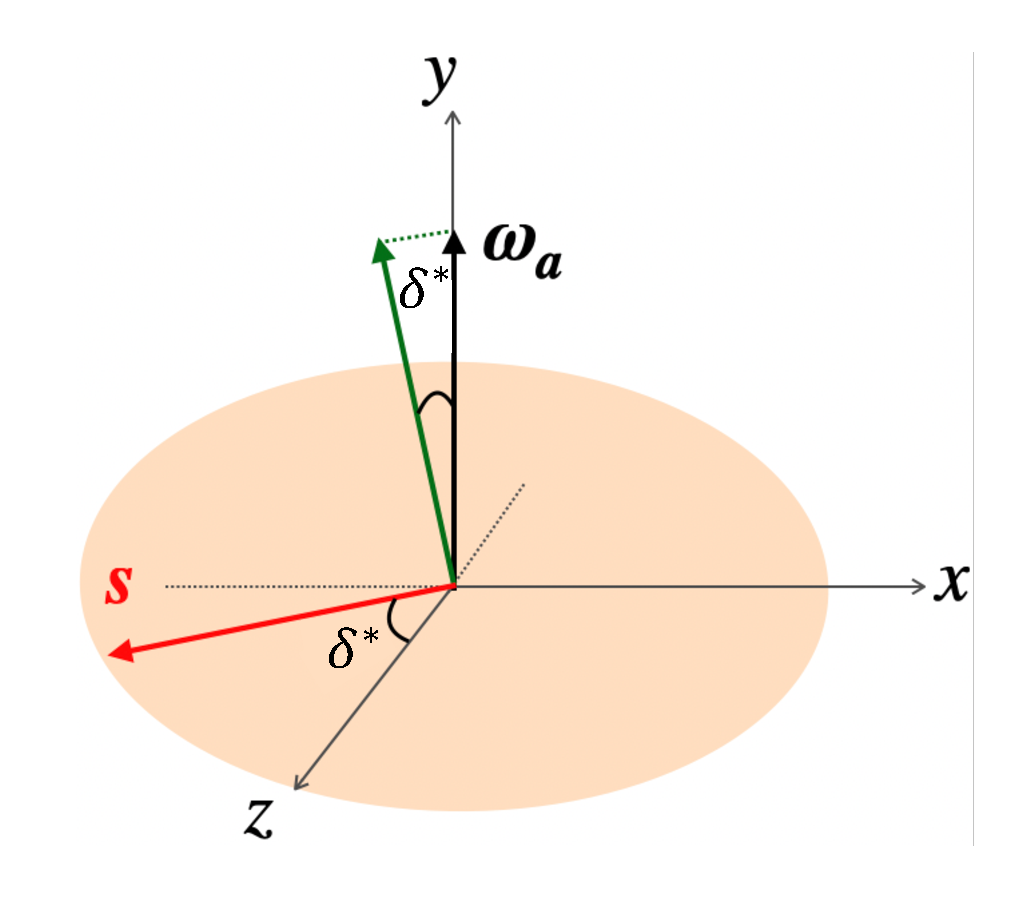
\includegraphics[trim={0 0 0 0},clip,width=0.49\textwidth]{Images/Chapter4/BzTilt2.pdf}\label{subfig:BzTilt} } \hfill  
\subfloat[Radial field.]{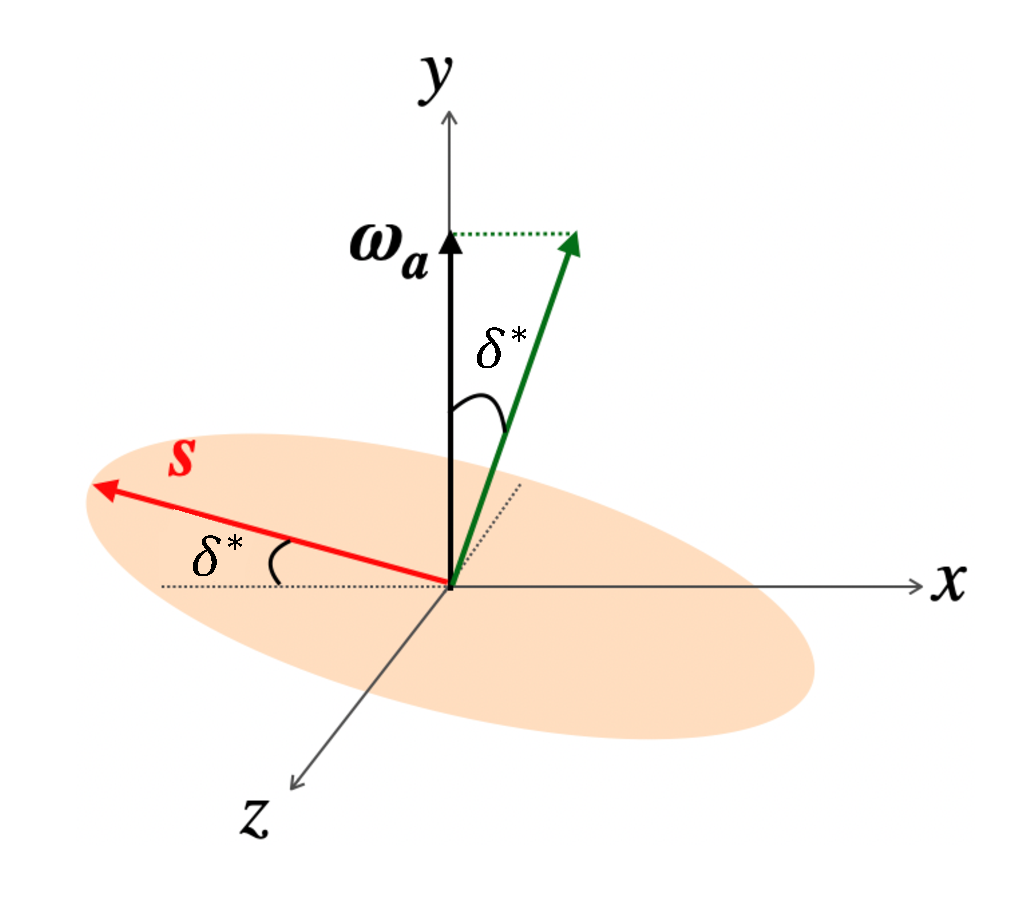
\includegraphics[trim={0 0 0 0},clip,width=0.49\textwidth]{Images/Chapter4/BrTilt2.pdf}\label{subfig:BrTilt} }
\caption{The tilt in muon spin precession plane resulting from: (a) a non-zero longitudinal field component; (b) a non-zero radial field component. Note that the radial field results a tilt in same direction as would be caused by a muon EDM, as shown in Figure \ref{subfig:EDMTilt}. Images courtesy of R. Chislett \cite{BeckyGeometry}.}
\label{fig:Tilt2}
\end{figure}
%

\section[The required precision of a radial field measurement]{The required precision of a radial field measurement}\label{sec:BrPrecision}

The required precision of a radial field measurement is governed by the statistical limit for sensitivity to an EDM signal. For any finite dataset, the statistical uncertainty will at some point overcome the systematic uncertainty caused by a radial field. At this point, no improvement in the total uncertainty can be made by improving the uncertainty on the radial field. Examples of the statistically limited EDM sensitivity against the radial field uncertainty are illustrated in Figure \ref{fig:BrUnc}, courtesy of D. Vasilkova \cite{DominikaCMJuly2021}. The case for a muon EDM measurement made using a dataset of one hundred million high quality tracks, approximately comparable to the size of the Run-1 dataset, is shown in Figure \ref{subfig:BrUncRun-1}. This indicates that the radial field uncertainty for an EDM search in Run-1 must be $\leq10$ ppm. For the integrated E989 dataset, consisting of billions of tracks, a precision of $\leq1$ ppm is required, as shown in Figure \ref{subfig:BrUncTot}. 

\begin{figure}[t!]
% \centering{}
\subfloat[One hundred million tracks.]{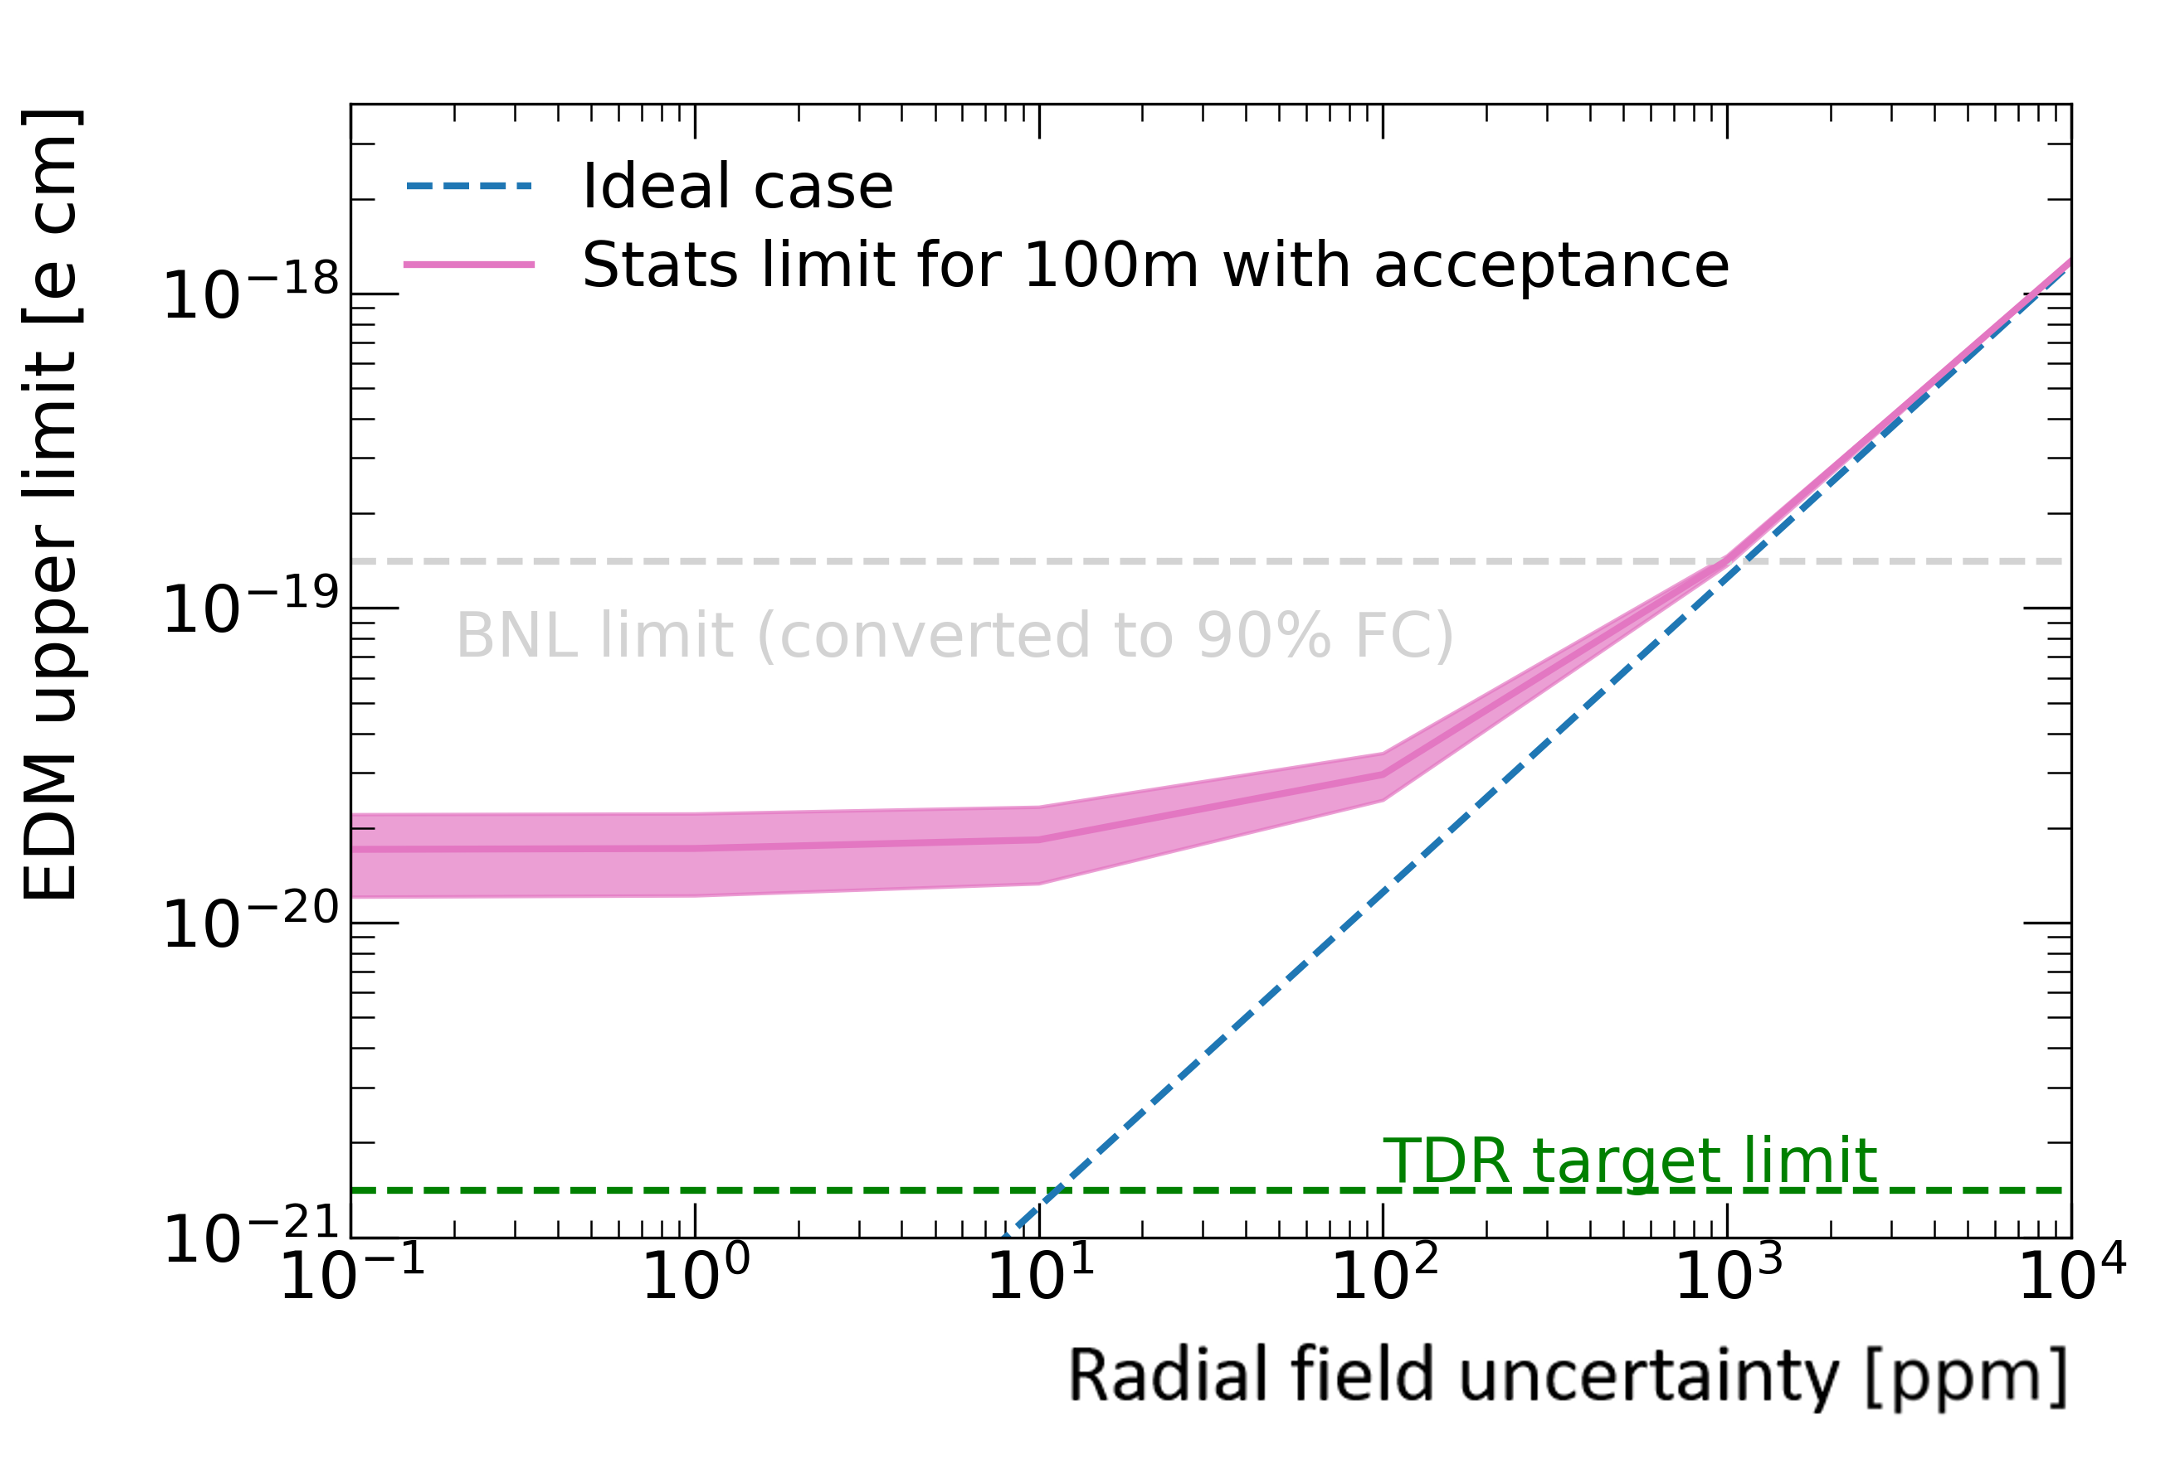
\includegraphics[trim={0 0 0 0},clip,width=0.47\textwidth]{Images/Chapter4/BrUncRun-1.png}\label{subfig:BrUncRun-1} }%\hfill
\subfloat[One and ten billion tracks.]{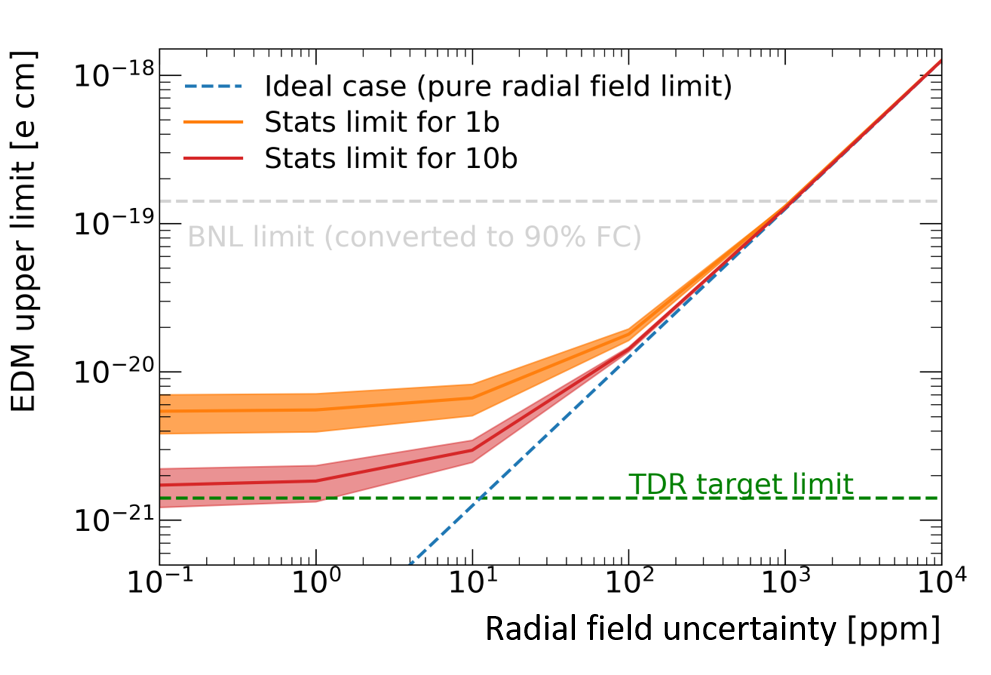
\includegraphics[trim={0 0 0 0},clip,width=0.47\textwidth]{Images/Chapter4/BrUncTotal.png}\label{subfig:BrUncTot} }
\caption{The upper limit on a muon EDM versus the uncertainty on a radial field measurement for: (a) one hundred million tracks, which is comparable to the E989 Run-1 dataset; (b) one to one hundred billion tracks, which is comparable to the target integrated dataset. For Run-1, the target precision for a radial field measurement is $\leq10$ ppm, while for the integrated dataset it is $\leq1$ ppm. Images courtesy of D. Vasilkova \cite{DominikaCMJuly2021}.}
\label{fig:BrUnc}
\end{figure}

\section{The distortion of the vertical closed orbit}\label{sec:VCOD}

A radial field would not only produce a tilt in the spin precession plane, but would also modify the average vertical beam position, $\langle y \rangle$, due to the Lorentz force. Counteracting this effect is vertical electric field from the ESQs\footnote{The electrostatic quadrupoles, introduced in Chapter \ref{chap:3} \ref{sec:ESQs}.}, which pushes the beam back towards the centre of the storage region so that an equilibrium position is reached. The resulting value of $\langle y \rangle$ depends on the size of the vertical ESQ potential difference, $V$, and $B_{r}$. The interaction between $V$, $B_{r}$, and $\langle y \rangle$ is central to the work presented in this chapter, as it may be exploited to make a measurement of $B_{r}$.

The interplay between the radial field and the ESQs is referred to as the distortion of the vertical closed orbit\footnote{The distortion of the closed orbit having been introduced in Chapter \ref{chap:3} Section \ref{subsec:COD}.} due to a magnetic skew dipole \cite{BillNote2020}, and is described by the summation
%
\begin{equation} 
  y(\theta) \approx \sum_{N=0}^{\infty} \frac{R_{0}}{B_{0}} \frac{(B_{rcN}\cos(N\theta)+B_{rsN}\sin(N\theta))}{N^{2}-n},
  \label{eqn:BVCOD}
\end{equation}
%
where $\theta$ is the azimuthal angle around the ring, $R_{0}$ is the ideal storage radius (7112 mm), $B_{0}$ is the dominant vertical magnetic dipole field, the $B_{r s,c}$ terms represent orthogonal components of the radial magnetic field, and $n$ is the ESQ field index, given by Equation \ref{eqn:FieldIndex}. For illustration, the simulated variation in $\langle y \rangle$ as a function of ring azimuth is shown in Figure \ref{fig:ClosedOrbitSim}. Expanding Equation \ref{eqn:BVCOD} gives
%
\begin{equation} 
  y(\theta) \approx \frac{R_{0}}{B_{0}} \left[ -\frac{B_{r,N=0}}{n} + \frac{B_{r,N=1}\cos(\theta-\phi_{1})}{1-n} + \frac{B_{r,N=2}\cos(2\theta-\phi_{2})}{4-n} + ... \right],
  \label{eqn:BVCODExpansion}
\end{equation}
%
where the phase shifts, $\phi_{N}$, are introduced by the absorption of the sine terms. The $N>0$ terms cancel when $\langle y \rangle$ is observed simultaneously around the ring, which in practice means taking the average position as measured over all calorimeters; a technique described in detail the following section. In this case, only the $N=0$ term remains, leaving the linear relationship % between $\langle y \rangle$, $\langle B_{r, N=0} \rangle$, and $n$:
%
\begin{equation} 
  \langle y \rangle = \frac{R_{0}}{vB_{0}} \frac{\langle B_{r} \rangle}{n} = \frac{\langle B_{r} \rangle}{\kappa}.
  \label{eqn:ZerothOrder}
\end{equation}
%
Furthermore, since $\kappa$ is proportional to $V$, the above expression may be simplified to give the relationship 
%
\begin{equation} 
  \langle y \rangle \propto \frac{\langle B_{r} \rangle}{V}, 
  \label{eqn:ZerothOrderSimple}
\end{equation}
%
which is central to the measurements presented in this chapter.

\begin{figure}[t!]
\centering{}
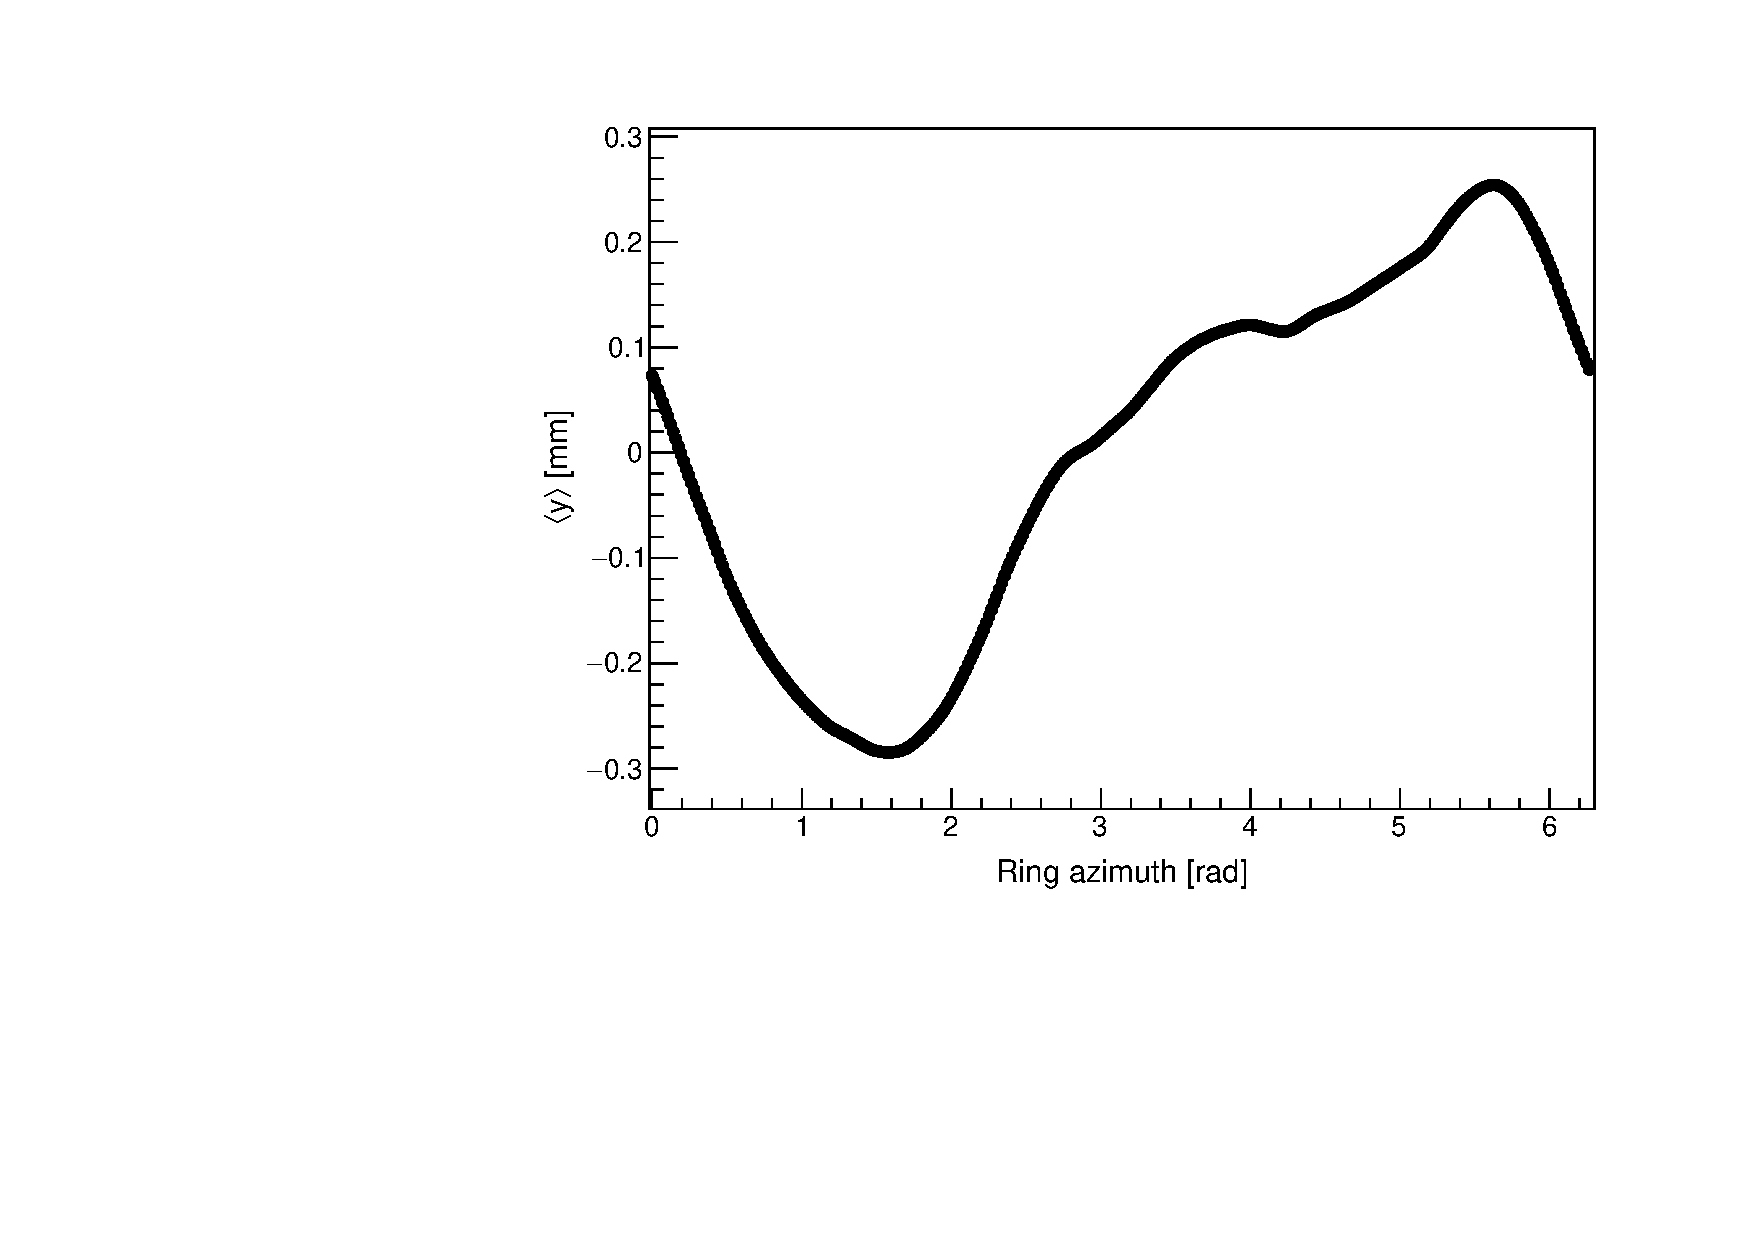
\includegraphics[trim={0 0 0 0},clip,width=0.65\textwidth]{Images/Chapter4/ClosedOrbitSim.pdf}
\caption{The variation in average vertical beam position as a function of ring azimuthal angle, from a simulation of the distortion of vertical closed orbit due to a magnetic skew dipole. Simulation data courtesy of D. Tarazona \cite{Tarazona}.}
\label{fig:ClosedOrbitSim}
\end{figure}

As an additional detail, simultaneously measuring $\langle y \rangle$ around the full ring azimuth also simplifies the influence of an additional distortion arising from misalignment of the ESQs. This phenomenon is referred to as the distortion of the vertical closed orbit due to an electric skew dipole, and is described, in a manner similar to Equation \ref{eqn:BVCOD}, by
%
\begin{equation} 
  y(\theta) \approx \sum_{N=0}^{\infty} \frac{R_{0}}{cB_{0}} \frac{(E_{ycN}\cos(N\theta)+E_{ysN}\sin(N\theta))}{N^{2}-n},
  \label{eqn:EVCOD}
\end{equation}
%
where $R_{0}/cB_{0} = n / \kappa$ by Equation \ref{eqn:FieldIndex}. If the $E_{y c,s}$ terms arise from ESQ misalignment then they will scale with $V$, as will $\kappa$. This makes the ratio $E_{y}/\kappa$ a constant. Expanding the summation, absorbing the sine terms with phase shifts as with Equation \ref{eqn:BVCODExpansion}, and defining $E_{y}/\kappa$=$E_{y}^{\prime}$ gives
%
\begin{equation} 
  y(\theta) \approx -E_{y0}^{\prime} + \frac{n}{1-n}E_{y1}^{\prime}\cos(\theta-\phi_{E,1}) + \frac{n}{4-n} E_{y1}^{\prime}\cos(2\theta-\phi_{E,2})+ ...
  \label{eqn:EVODExpansion}
\end{equation}
%
As with Equation \ref{eqn:BVCODExpansion}, the $N>0$ terms cancel when taking the average $\langle y \rangle$ around the full ring azimuth, leaving the constant $-E_{y0}^{\prime}$. Importantly, this means that the dependence of the ring average $\langle y \rangle$ on $V$ has no contribution from ESQ misalignment, and is driven exclusively by $\langle B_{r} \rangle$, according to Equation \ref{eqn:ZerothOrderSimple}.

\section{Measurement technique}\label{sec:MeasuringBr}

\subsection{Measuring the background radial field}\label{sec:MeasuringBr}

% \myworries{Calorimeters! Surface coils!}

The average radial field, $\langle B_{r} \rangle$, has two contributions: the average field applied by the surface correction coils (SCCs)\footnote{The SCCs are described in detail in Chapter \ref{chap:3} Section \ref{sec:Field}.}, $\langle B_{r}^{a} \rangle$, and an unknown average background field, $\langle B_{r}^{b} \rangle$, so that 
%
\begin{equation} 
  \langle B_{r} \rangle = \langle B_{r}^{a}\rangle + \langle B_{r}^{b}\rangle.
  \label{eqn:TotalBr}
\end{equation}
%
In the case where the total field is zero, $\langle B_{r}^{b}\rangle$ must be equal in magnitude and opposite in sign to $\langle B_{r}^{a} \rangle$, which is a known quantity, as follows
%
\begin{equation} 
  \langle B_{r} \rangle = 0 \rightarrow \langle B_{r}^{a}\rangle = - \langle B_{r}^{b}\rangle.
  % \label{eqn:TotalBr}
\end{equation}
%
The challenge is then to find the point at which $\langle B_{r} \rangle = 0$. Following the relationship given by Equation \ref{eqn:ZerothOrderSimple}, this is possible by performing a series of ESQ scans of $V$ over a range of SCC $\langle B_{r}^{a} \rangle$ values, measuring the ring average $\langle y \rangle$ by taking the mean vertical hit position as measured by all calorimeters at each set point. Calorimeter hit position is often referred to as `cluster position' in E989, and is calculated by taking an energy weighted average of the central positions of crystals in cluster of hits. Detailed discussion on the formation of calorimeter clusters and the calculation of cluster position may be found in \cite{Fienberg}. An example of the distribution for vertical cluster positions, in this case for the Run-1a dataset, is given by Figure \ref{fig:CaloAvgYPlot}.

\begin{figure}[t!]
\centering{}
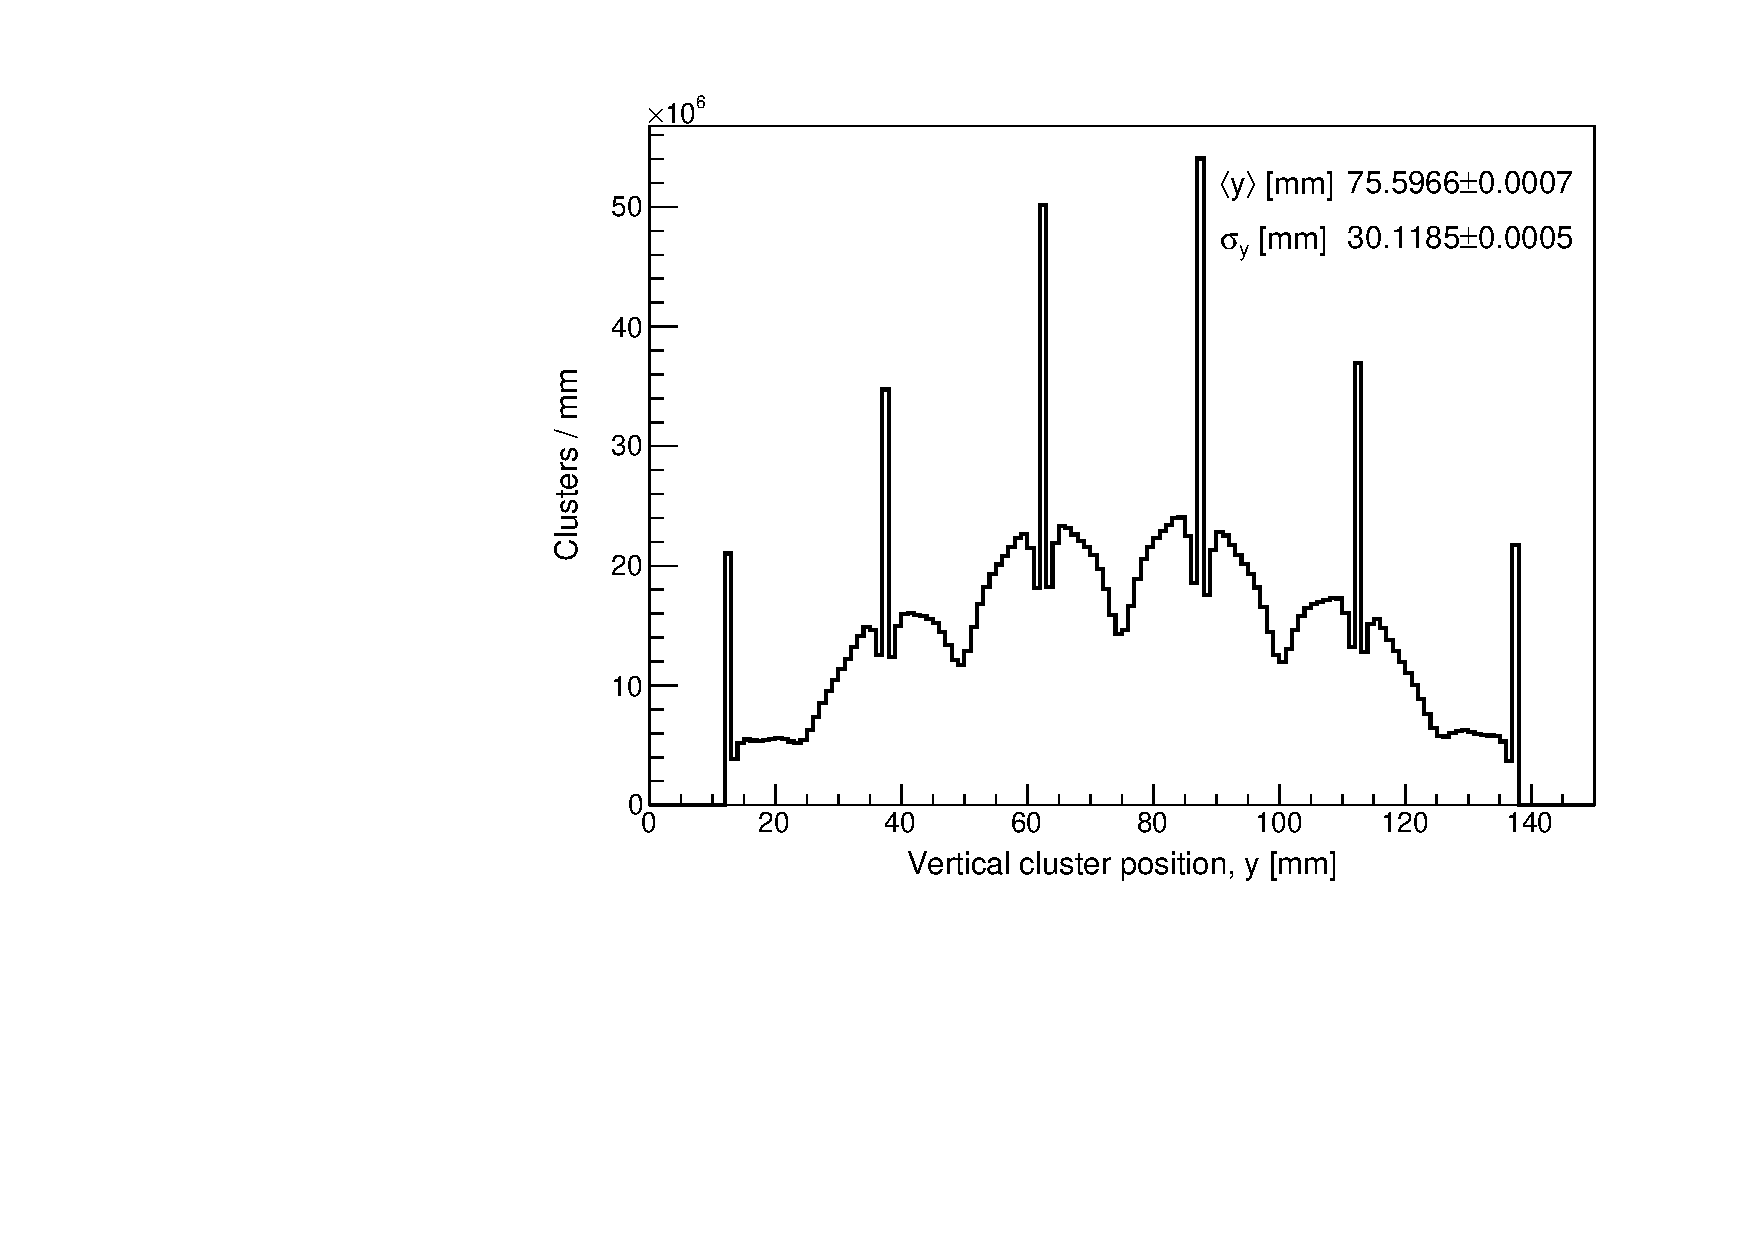
\includegraphics[trim={0 0 0 0},clip,width=0.65\textwidth]{Images/Chapter4/CaloAvgYPlot.pdf}
\caption{The distribution of vertical cluster positions for all calorimeters in the Run-1a dataset, where the mean, $\langle y \rangle$, is taken as a proxy for the ring average vertical beam position. The peaks in the distribution correspond to clusters where a single crystal was hit.}
\label{fig:CaloAvgYPlot}
\end{figure}

This technique is most easily described with the aid of a toy model of the measurement, summarised in Figure \ref{fig:ToyMonteCarloFits}. In this example, there is an injected $\langle B_{r}^{b}\rangle$ of 8 ppm, twenty four set-points, an inputted statistical uncertainty on $\langle y \rangle$ drawn from Run-1 data (discussed further Section \ref{sec:PlanningBr}). Uncertainties associated with $V$ and $B_{r}^{a}$ are, at present, neglected in the work presented in this chapter; however, current best estimates give small uncertainties of $\sim$0.1 kV and $\sim$3\% respectively \cite{VoltageError}\cite{SimonRadialFieldTalk}. Figure \ref{subfig:ToyQuadScans} illustrates the ESQ scans of $V$, and Figure \ref{subfig:ToyFieldFit} demonstrates how the gradients of linear fits made to those scans, which are proportional to the $\langle B_{r} \rangle$ by Equation \ref{eqn:ZerothOrderSimple}, vary with $\langle B_{r}^{a} \rangle$. The point at which $\langle B_{r} \rangle = 0$ is found by evaluating a linear fit to this secondary plot, where $\langle B_{r}^{b} \rangle$ is equal in magnitude and opposite in sign to the $x$-intercept of the fit. If the parameters of this fit consist of a gradient $m$ and a $y$-intercept $c$, then the uncertainty on the $x$-intercept -- the uncertainty on $\langle B_{r}^{b} \rangle$ -- is given by 
%
\begin{equation}
  \delta \langle B_{r}^{b} \rangle = \langle B_{r}^{b} \rangle \sqrt{ \left(\frac{\delta m}{m}\right)^{2} + \left(\frac{\delta c}{c}\right)^{2} - \frac{2}{mc}\sigma_{mc} },
\label{eqn:BackgroundBrUnc}
\end{equation}
%
where $\sigma_{mc}$ is the covariance of the fit parameters $m$ and $c$ \cite{Taylor}. A full derivation of Equation \ref{eqn:BackgroundBrUnc} is given in Appendix \ref{app:Unc} Section \ref{app:Brb}. Finally, once $\langle B_{r}^{b} \rangle$ has been measured, the SCC currents may be adjusted so that $\langle B_{r}^{a} \rangle = - \langle B_{r}^{b} \rangle$, setting $\langle B_{r} \rangle$ to zero. 

\begin{figure}[t!]
\centering{}
\subfloat[Toy ESQ/SCC scans.]{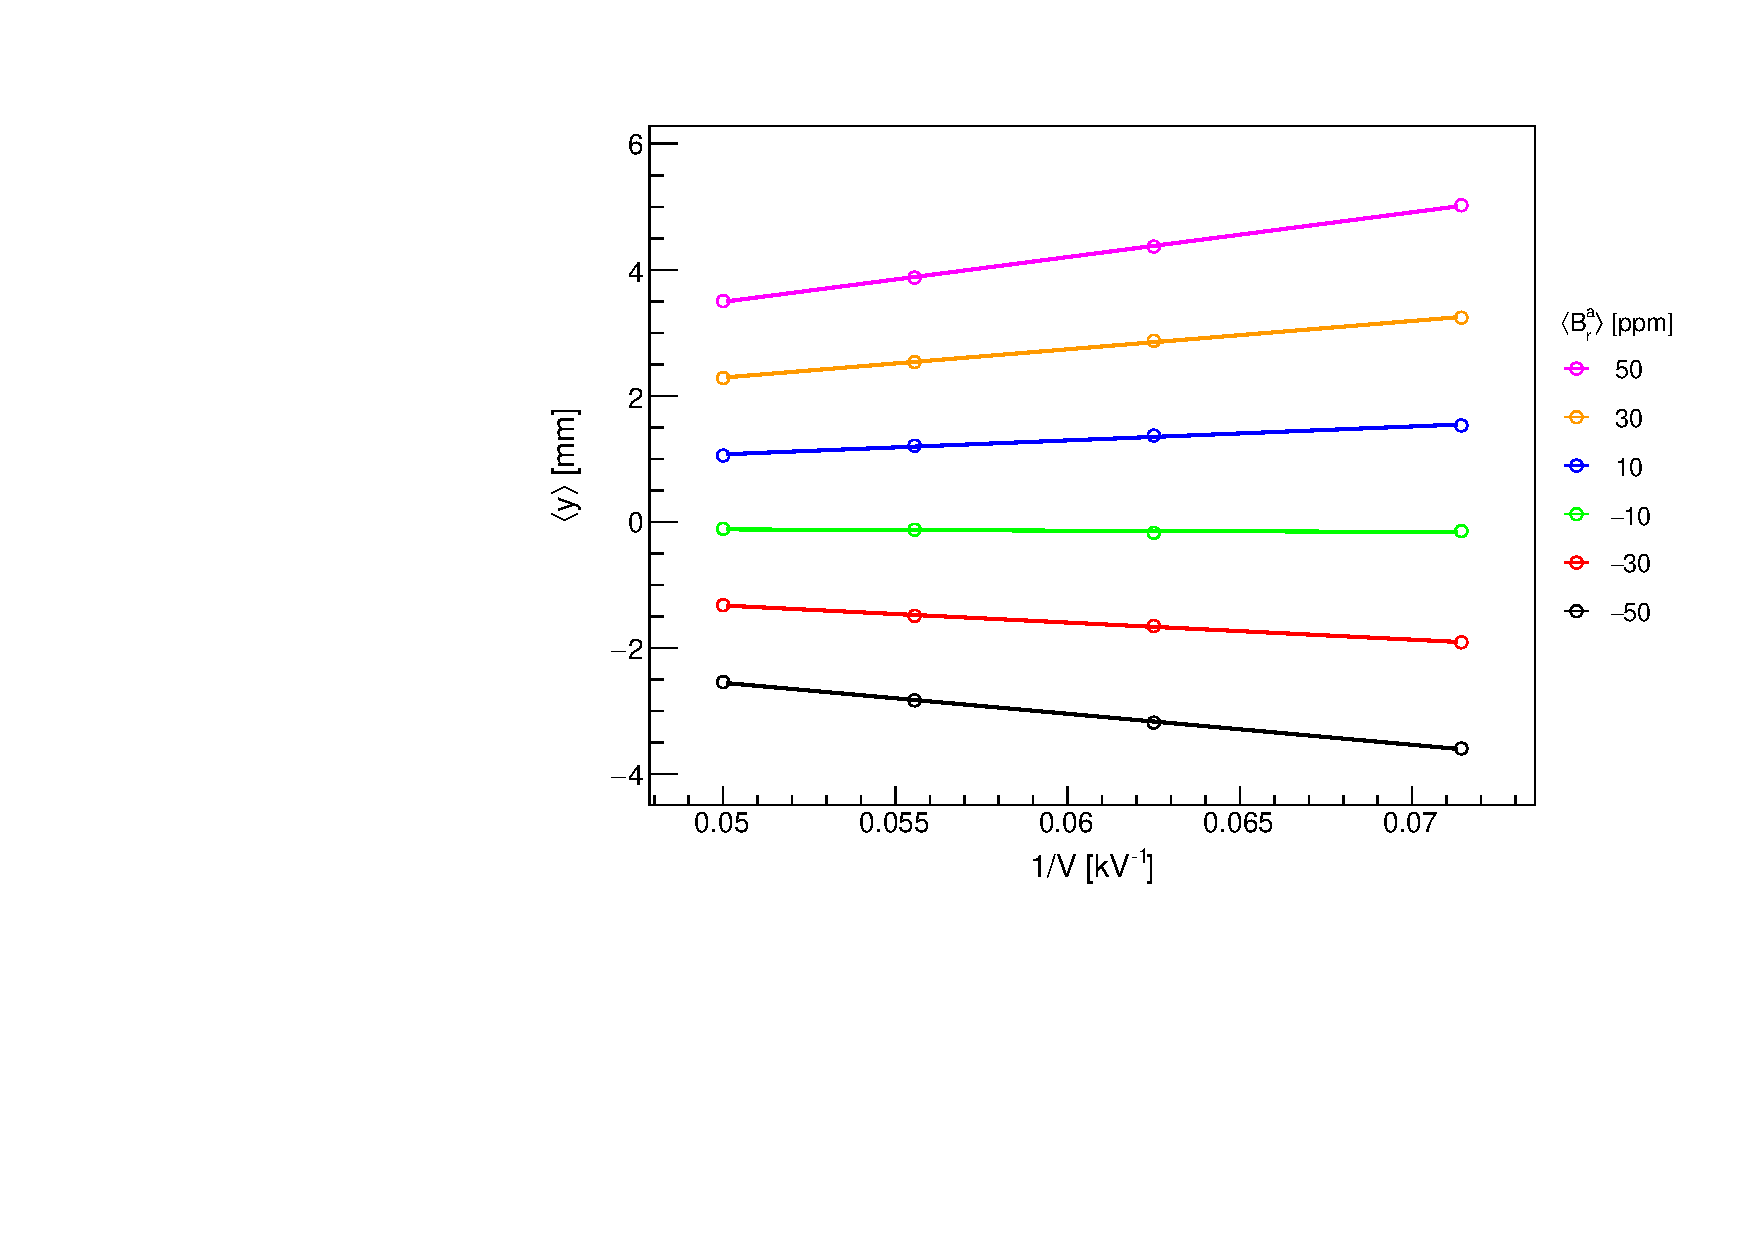
\includegraphics[trim={0 0 0 0},clip,width=0.49\textwidth]{Images/Chapter4/QuadScans_NSUBRUN_75_NEXP_0.pdf}\label{subfig:ToyQuadScans} }%\hfill
\subfloat[Toy $\langle B_{r}^{b} \rangle$ fit.]{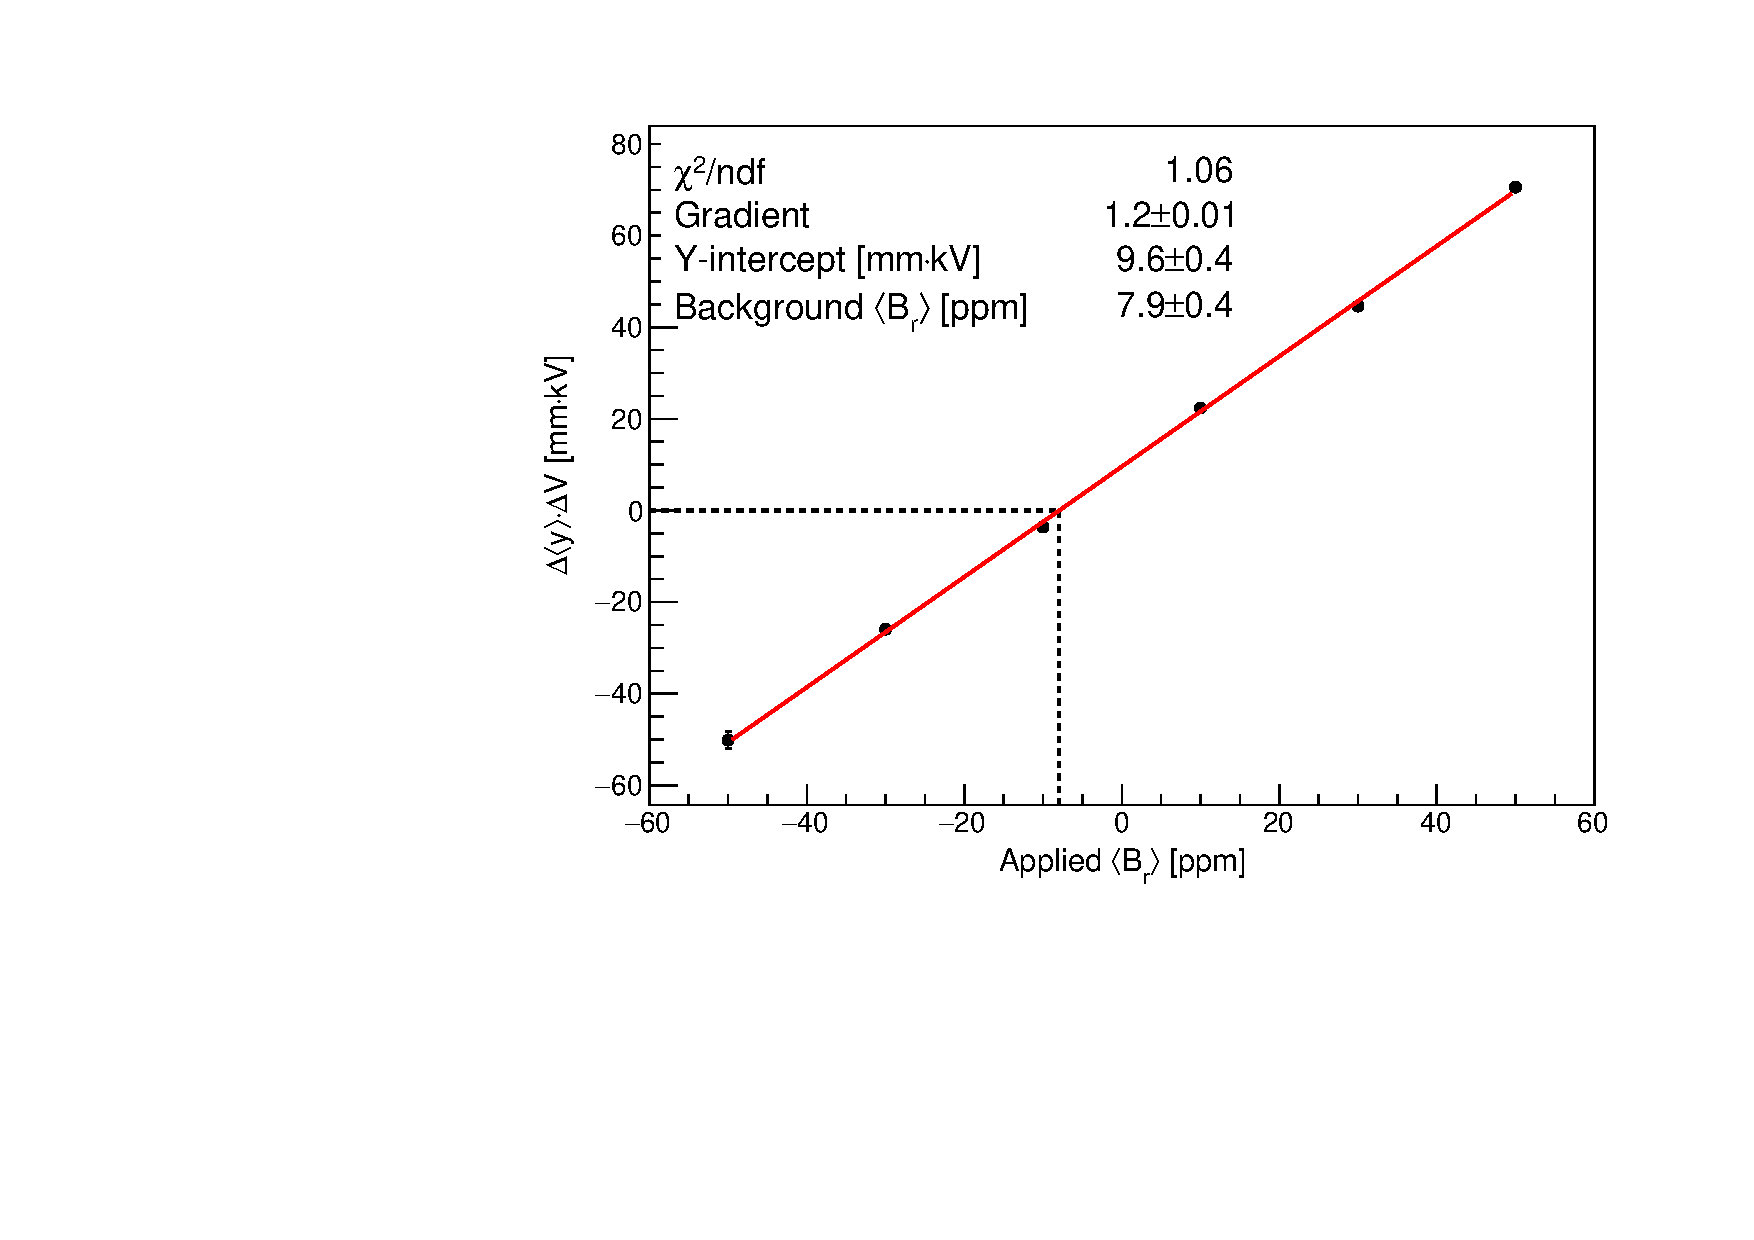
\includegraphics[trim={0 0 0 0},clip,width=0.49\textwidth]{Images/Chapter4/FieldFit_NSUBRUN_100_NEXP_738.pdf}\label{subfig:ToyFieldFit} }
\caption{Fits for a toy radial field measurement with twenty four set-points and an injected $\langle B_{r}^{b} \rangle$ of 8 ppm. The measured result shows good agreement with the true value, and the uncertainty is less than the target of 1 ppm.}
\label{fig:ToyMonteCarloFits}  % \SI{17.1}{\micro\metre} (equivalent to 2.87 million CTAGs or 75 sub-runs per ESQ setting)
\end{figure}

\subsection{Practical considerations}\label{sec:PlanningBr}

The aforementioned toy model, while useful for purposes of demonstration, was created primarily to provide a means of preparing the practical aspects of the measurement, such as: the values of the set-points, the number of set-points, and the total amount of beam time required to reach the target statistical precision of $\leq1$ ppm stated in Section \ref{sec:BrPrecision}.

In the toy model, the uncertainty on the average vertical cluster position per set-point, $\delta \langle y \rangle$, is assigned based on statistical uncertainties sampled from Run-1 data. For example, the toy measurement shown in Figure \ref{fig:ToyMonteCarloFits} possesses an inputted $\delta \langle y \rangle$ of \SI{17.1}{\micro\metre} (equivalent to 2.87 million CTAGs\footnote{A CTAG, or calorimeter tag, is a measure of the number of calorimeter hits recorded over a certain time and energy range. It is used as a proxy for muon storage in E989 \cite{CTAG}.} or 75 subruns\footnote{A subrun is a subset of a run: a period of data collection defined by MIDAS DAQ system described in Chapter \ref{chap:3} Section \ref{sec:Computing}.}). The central value, $\langle y \rangle$, is randomly drawn from a Gaussian distribution with a mean calculated by Equation \ref{eqn:ZerothOrder}, and a width equal to $\delta\langle y \rangle$. Many trial measurements may be performed to populate a distribution of fit uncertainties, $\delta \langle B_{r}^{b} \rangle$, the mean of which may be taken as the statistical precision associated with a particular configuration of set-points at some $\delta\langle y \rangle$. 

\begin{figure}[t!]
\centering{}
\subfloat[Storage fraction vs. $\langle B_{r}^{a} \rangle$.]{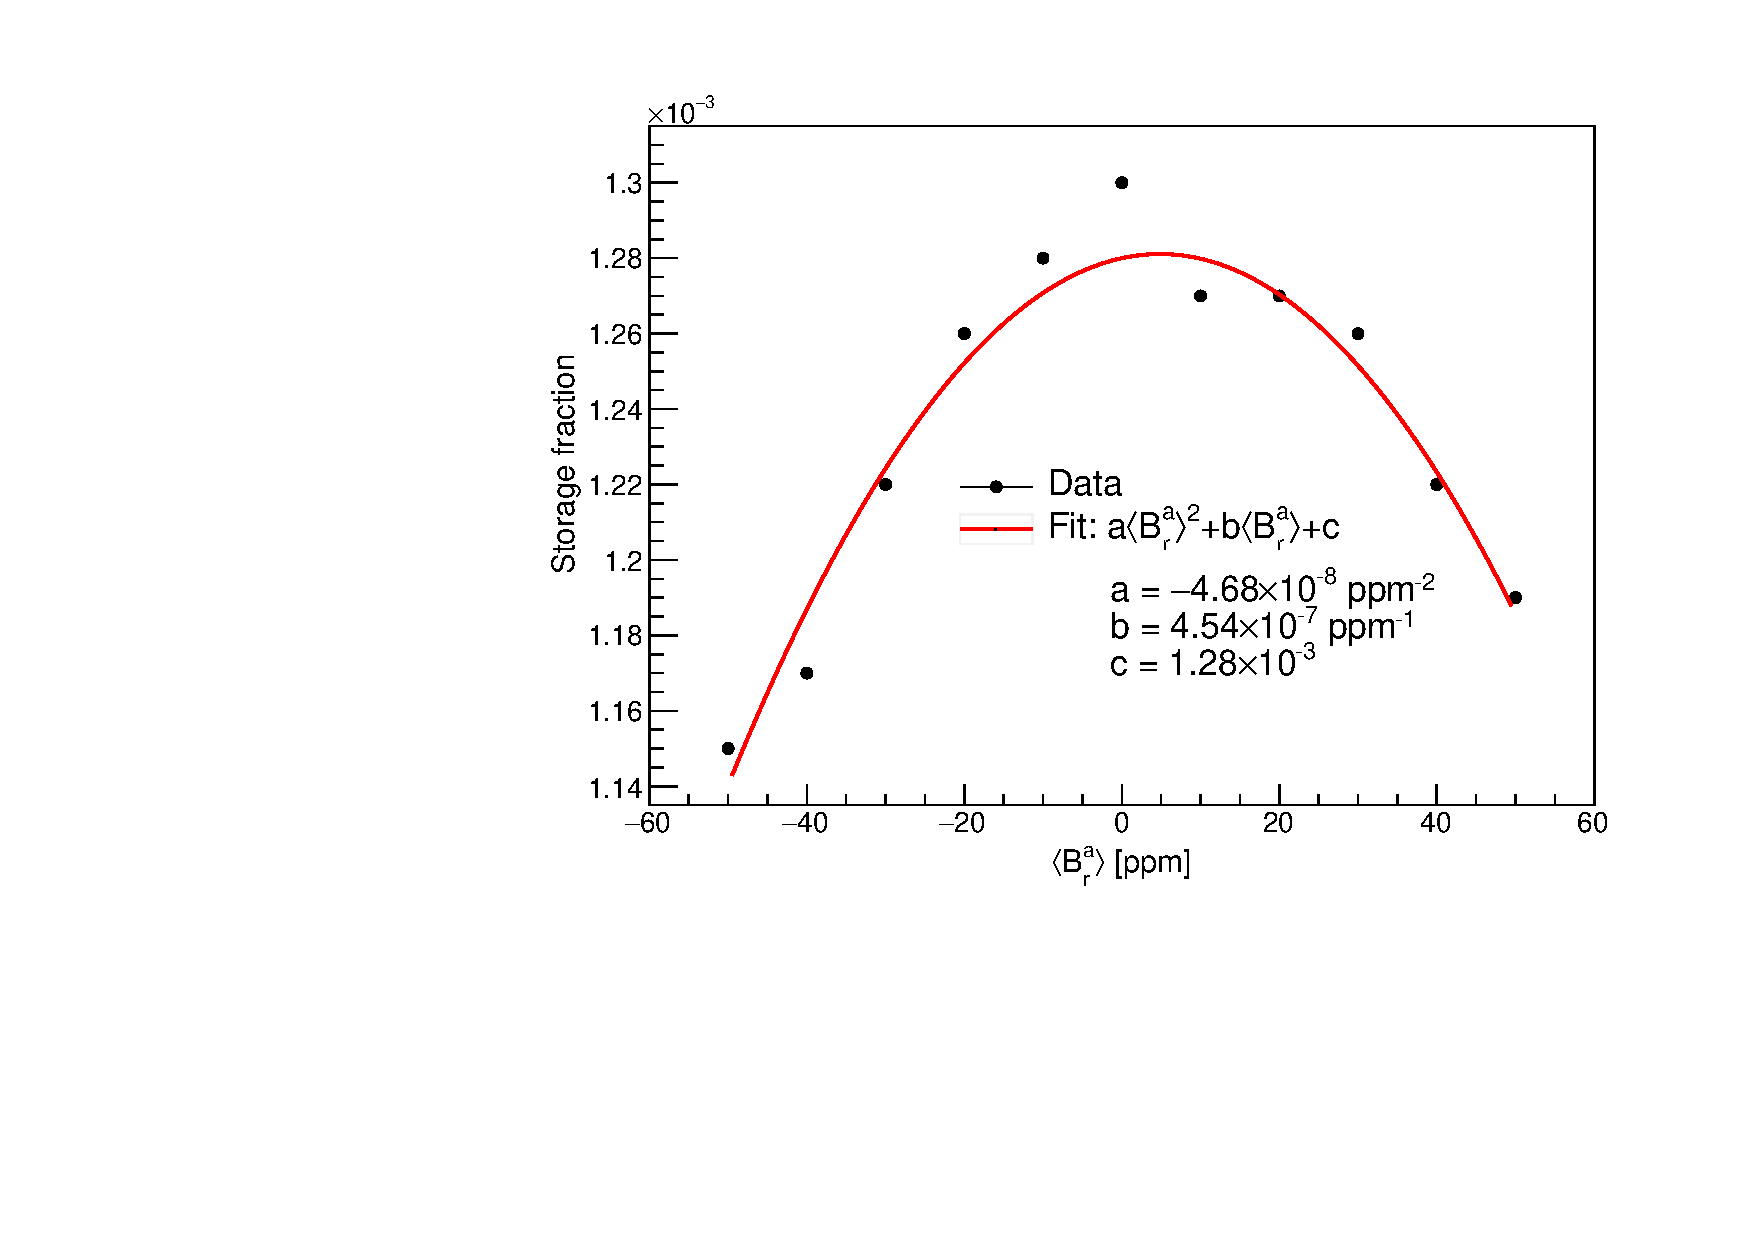
\includegraphics[trim={0 0 0 0},clip,width=0.48\textwidth]{Images/Chapter4/SCCStorage.pdf}\label{subfig:SCCStorage} } \hfill
\subfloat[Storage fraction vs. $V$.]{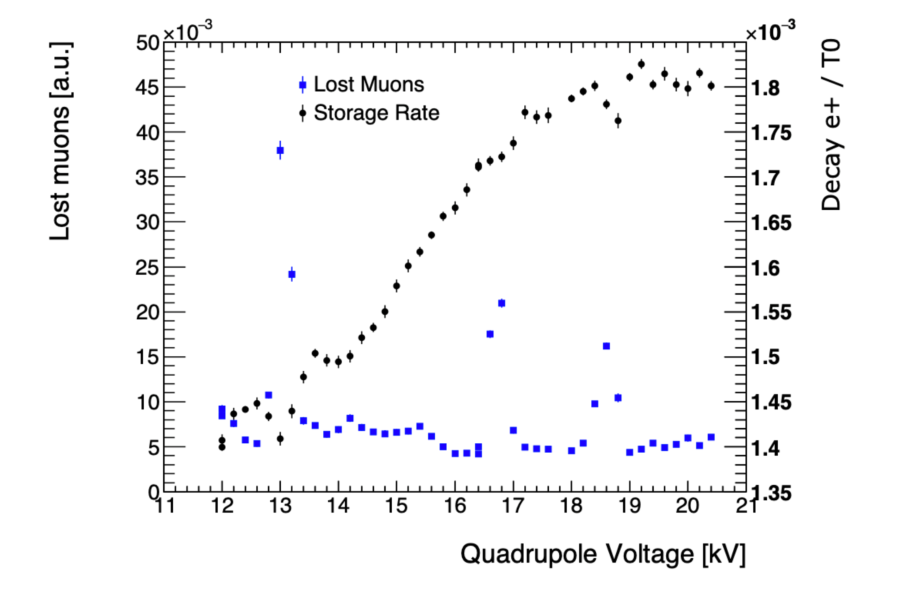
\includegraphics[trim={0 0 0 0},clip,width=0.49\textwidth]{Images/Chapter4/ESQStorage.pdf}\label{subfig:ESQStorage}}
\caption{The change in muon storage fraction when adjusting (a) SCC $\langle B_{r} \rangle$ set-points, and (b) ESQ voltages  . The minimum storage at 14 kV and $-50$ ppm is $\sim$300 CTAGs/fill. Images courtesy of P. Winter and A. Tewsley-Booth \cite{RadialFieldScanElog}, and E. Barlas-Yucel \cite{ESQStorage}.}
\label{fig:Storage}
\end{figure}

The set-point configuration was chosen to give the widest range of values possible, without compromising on muon storage, based on the variation in storage over a range of $\langle B_{r}^{a} \rangle$ and $V$ shown in Figure \ref{fig:Storage}. Additionally, the maximum ESQ voltage was limited to $19.5$ kV, according to the tolerances of the system. This chosen configuration utilised a total number of set-points, $N_{\text{set}}$, of twenty four, with: voltages of 14, 16, 18, and 19.5 kV; and applied radial fields of $-50$, $-30$, $-10$, 10, 30, and 50 ppm. Using this configuration, 1000 trials of the toy measurement were performed with varying levels of $\delta \langle y \rangle$, where the mean fit uncertainties are distributed against CTAGs per setting in Figure \ref{fig:BrErr_and_BrResRMS}. The widths of the truth residual distributions for each value of $\delta \langle y \rangle$ are also overlaid as a cross-check, showing good agreement. All input values of $\delta \langle y \rangle$ produce a results with $\delta \langle B_{r}^{b} \rangle < 1$ ppm. From this, it may be inferred that the minimum total number of CTAGs, $N_{\mu}$, required to reach $\leq1$ ppm is $\sim9.5\times10^{5}$ (or 25 subruns). Referring again to Figure \ref{fig:Storage}, the required beam-time of the measurement was calculated based on a conservative estimate of the average muon storage rate over the full measurement, $R_{\mu}$, of $\sim$300 CTAGs per fill at 11 Hz. The total measurement time, $t_{\text{tot}}$, may then be estimated, accounting for the time for adjustment between set-points, $t_{a}$, by 
%
\begin{equation}
  t_{\text{tot}} = N_{\text{set}}\cdot\left(\frac{N_{\mu}}{R_{\mu}} + t_{a}\right). %S_{\mu}}{}
  \label{eqn:BrTiming}
\end{equation}
%
This means that the minimum $t_{\text{tot}}$ required, with $t_{a}=5$ minutes, would be $\sim4$ hours. Fortunately, the time allocated for this measurement was $\leq12$ hours, making it possible to maximise the statistical precision by targeting $N_{\mu}=3.79\times10^{6}$ CTAGS (100 sub-runs, or $\sim$20 minutes beam-time) per set-point, or $t_{\text{tot}}\approx10$ hours, corresponding to an estimated precision of $\delta \langle B_{r}^{b} \rangle = 0.403$ ppm. As an essential additional note in the methodology, ESQ beam scraping (which moves the beam in the $x$-$y$ plane) was disabled for this measurement.

\begin{figure}[t!]
\centering{}
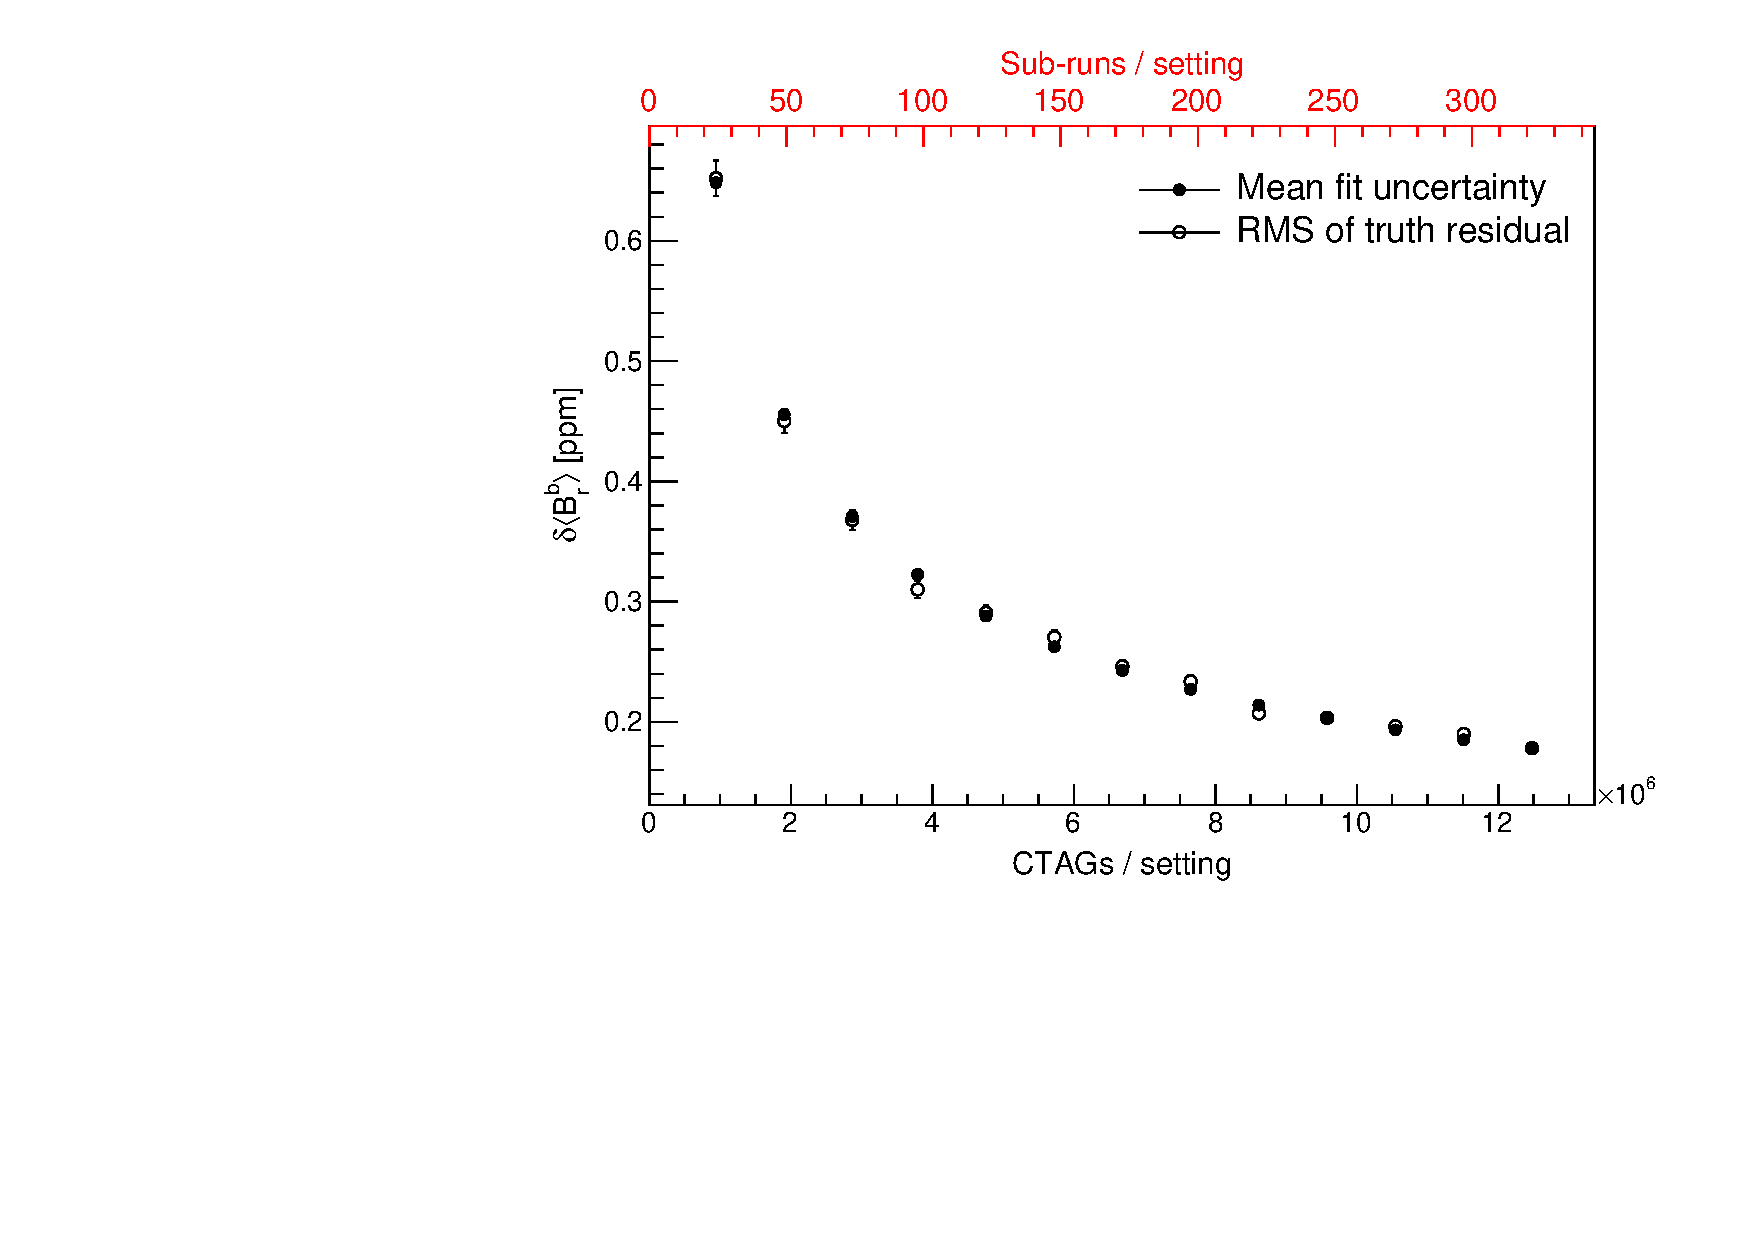
\includegraphics[trim={0cm 0cm 0cm 0cm},clip,width=0.65\textwidth]{Images/Chapter4/BrErr_and_BrResRMS_overlay.pdf}
\caption{The mean fit uncertainties and the widths of the truth residual distributions for 1000 trial measurements, using the same configuration of set-points shown in Figure \ref{fig:ToyMonteCarloFits}, graphed against CTAGs and subruns per setting. Data points at the same level of statistical uncertainty are consistent between the two distributions, and all values of $\delta \langle B_{r}^{b} \rangle$ are better than the target uncertainty of 1 ppm.}
\label{fig:BrErr_and_BrResRMS}
\end{figure}

\subsection{Extrapolating the results}

In the context of the muon EDM search, $\langle B_{r} \rangle$ must be known for all E989 datasets used in the analysis. Estimates of $\langle B_{r} \rangle$ can be made for any dataset by examining the change in $\langle y \rangle$, $\Delta \langle y \rangle$, relative to a reference position, $ \langle y \rangle_{\text{ref}}$, where $\langle B_{r}^{b} \rangle$ is known, given by
%
\begin{equation}
  \Delta \langle y \rangle = \langle y \rangle - \langle y \rangle_{\text{ref}}.
  \label{eqn:DeltaYRef}
\end{equation}
%
This may be converted into $\Delta \langle B_{r} \rangle$ by a constant conversion factor, $k$:
%
\begin{equation}
  \Delta \langle B_{r} \rangle = k \Delta \langle y \rangle.
  \label{eqn:RadialFieldChange}
\end{equation}
%
If $k$, and by extension, $\Delta \langle B_{r} \rangle$, is known, then $\langle B_{r} \rangle$ may be estimated according to 
% %
\begin{equation}
  \langle B_{r} \rangle = \Delta \langle B_{r} \rangle  + \langle B_{r}^{b} \rangle_{\text{ref}}.
  \label{eqn:AbsRadialField}
\end{equation}
%
The constant $k$ is found via an empirical method, where data from the radial field measurement is recycled to make linear fits to $\langle y \rangle$ against $\langle B_{r}^{a} \rangle$ for a range of voltages, the gradients of which are plotted against $1/V$, and the ensuing distribution is fitted with a straight line of the form
%
\begin{equation}
  \frac{\Delta \langle y \rangle}{\Delta \langle B_{r}^{a} \rangle} = \frac{m}{V} + c, 
  % \rightarrow \frac{\Delta \langle y \rangle}{k \Delta \langle y \rangle} = \frac{m}{V} + c \\
\end{equation}
%
where $m$ and $c$ are the gradient and $y$-intercept, and $\Delta \langle B_{r}^{a} \rangle = k \Delta \langle y \rangle $, from Equation \ref{eqn:RadialFieldChange}. Provided that $V$ is known in the dataset of interest, $k$ may be calculated by 
%
\begin{equation}
  k = \frac{1}{\frac{m}{V} + c}.
  \label{eqn:EmpricalConversionFactor}
\end{equation}
%
This approach may be conceptualised as an inversion of the procedure used to measure $\langle B_{r}^{b} \rangle$, and is demonstrated in practice in Section \ref{subsection:ExtrapolatingTheRadialField}. The uncertainty associated with $k$ is given by the expression
%
\begin{equation}
  \delta k = \sqrt{ \left(\frac{1}{Vk^{2}}\right)^{2}\cdot \delta m ^{2} 
  + \left(\frac{1}{k^{4}}\right)\cdot\delta c^{2}
  + \left(\frac{2}{Vk^{4}}\right)\cdot \sigma_{mc} }, 
\end{equation}\label{eqn:EmpricalConversionFactorError}
%
where $\sigma_{mc}$ is the covariance of the fit parameters $m$ and $c$ \cite{Taylor}. A full derivation for Equation \ref{eqn:EmpricalConversionFactor} is given in Appendix \ref{app:Unc} Section \ref{app:k}. 

\begin{figure}[t!]
\centering{}
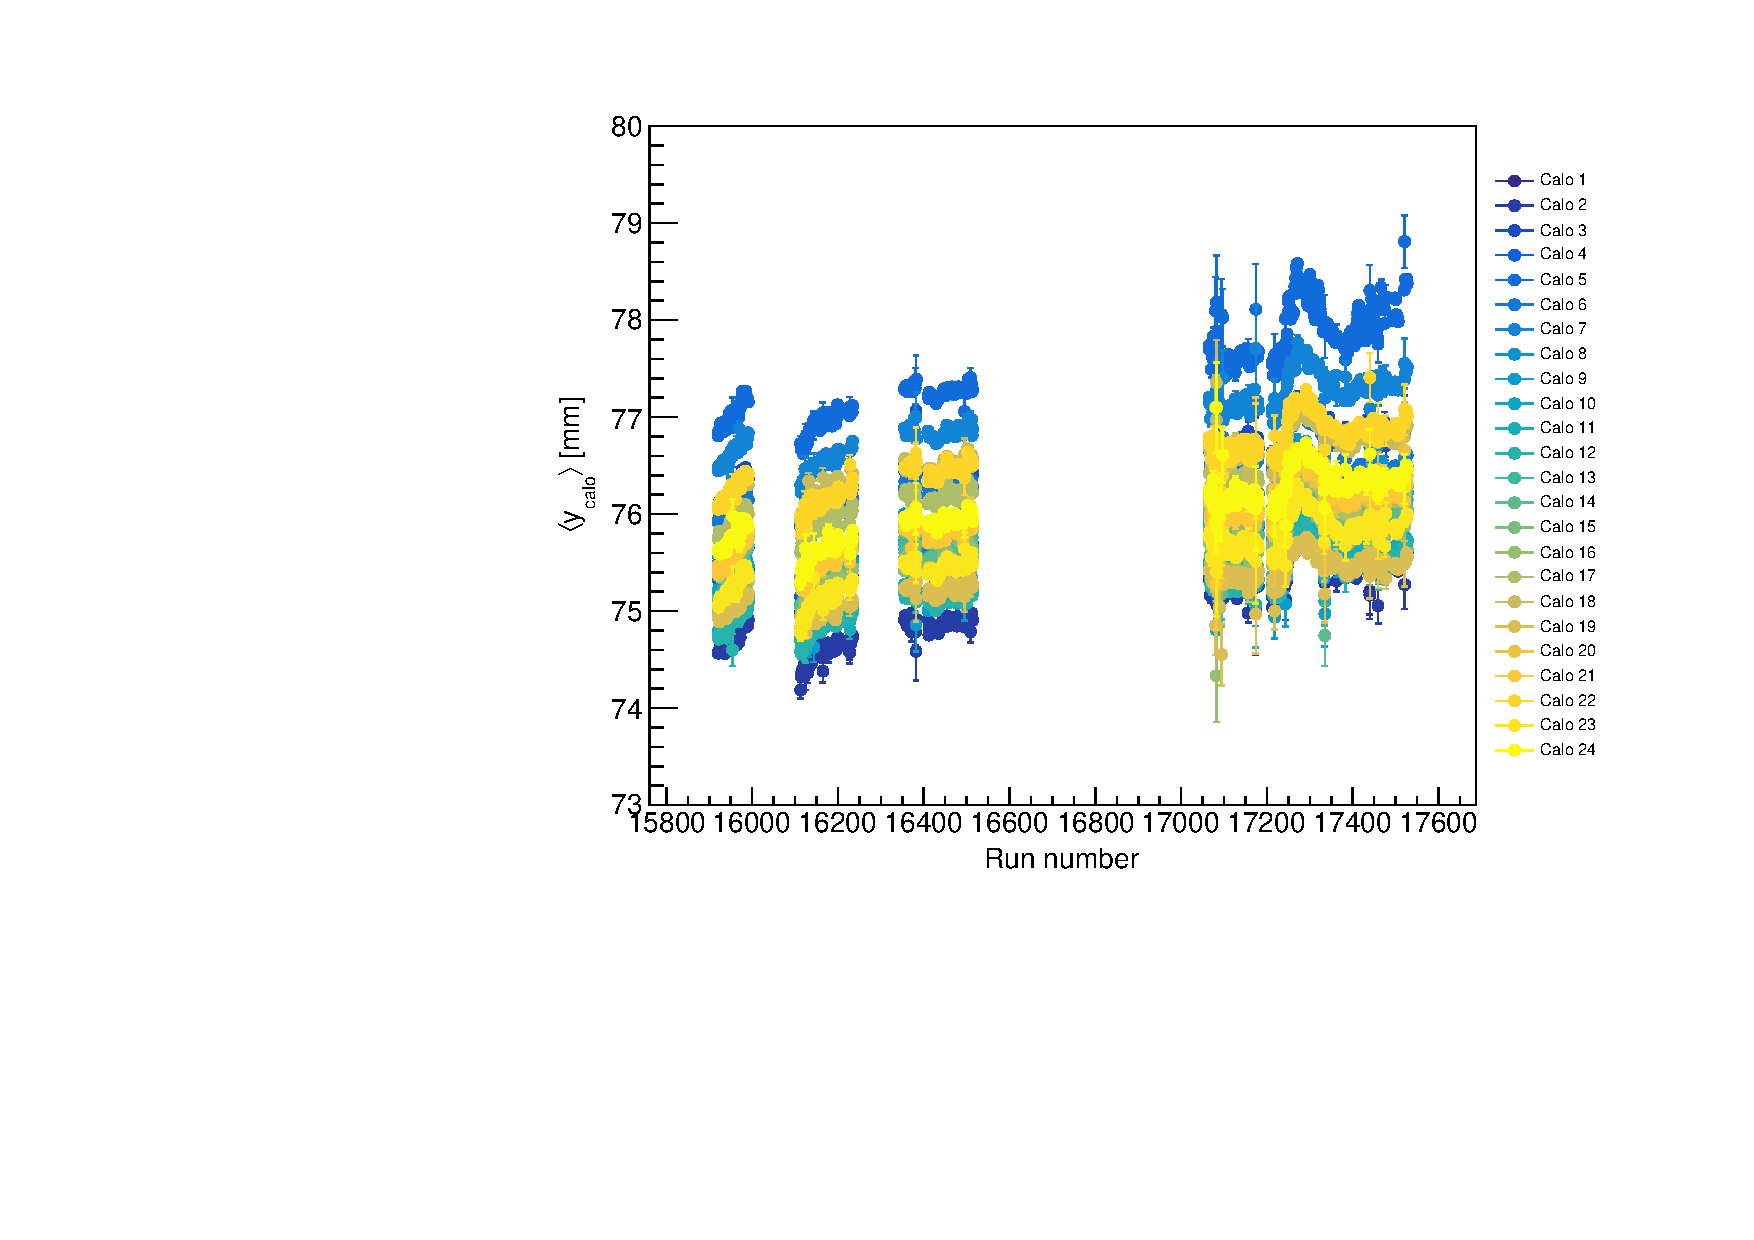
\includegraphics[trim={0 0 0 0},clip,width=0.65\textwidth]{Images/Chapter4/PerCaloYvsRun_Run1_15921_17527.pdf}
\caption{$\langle y \rangle$ per calorimeter in Run-1, where the four distinct datasets may be clearly seen. The differences in position between calorimeters is due to their relative misalignment, and the drift in position arises from a varying radial magnetic field caused by temperature fluctuations.}
\label{fig:PerCaloYvsRun_Run1}
\end{figure}  

The uncertainty on $\Delta \langle y \rangle$ receives contributions from statistical uncertainties on both the reference position and the measurement position, $\delta_{\text{stat}}$, the systematic uncertainty arising the potential changes in calorimeter alignment between the reference dataset and the dataset of interest, $\delta_{\text{align}}$, as well as the size of any drift in $\langle y \rangle$ over the dataset, $\delta_{\text{drift}}$. The necessity of accounting for $\delta_{\text{align}}$ and  $\delta_{\text{drift}}$ is obvious from the distribution of $\langle y \rangle$ per calorimeter, $\langle y_{\text{calo}} \rangle$, shown for Run-1 in Figure \ref{fig:PerCaloYvsRun_Run1}. The relative misalignment can be seen in the differences in vertical position between calorimeters. The drift in position, arising from a varying radial magnetic field, due to temperature fluctuations causing contraction and expansion of the magnet, is also clearly seen. $\delta_{\text{align}}$ is estimated by measuring the difference in vertical beam position reported by adjacent pairs of calorimeters in a particular dataset, taking the change in these differences compared to the reference position, and then taking the width of the resulting distribution as the uncertainty. $\delta_{\text{drift}}$ is taken to be the width of the distribution of $\langle y \rangle$ for a particular dataset. The total uncertainty on $\Delta \langle y \rangle$ is then the sum of these contributions in quadrature, so that
%
\begin{equation}
  \delta\Delta \langle y \rangle = \sqrt{\delta_{\text{stat}}^{2}+\delta_{\text{align}}^{2}+\delta_{\text{drift}}^{2}},
  \label{DeltaPositionUncertainty}
\end{equation}
%
where the uncertainty on $\Delta \langle B_{r} \rangle$ is given by
%
\begin{equation}
  \delta\Delta \langle B_{r} \rangle = \Delta \langle B_{r} \rangle \sqrt{ \frac{\delta \Delta \langle y \rangle}{\Delta \langle y \rangle}^{2} + \frac{\delta k}{k}^{2} }.
  \label{eqn:DeltaBrUncertainty}
\end{equation}
%
The absolute radial field uncertainty may then estimated by combining of Equation \ref{eqn:DeltaBrUncertainty} and the uncertainty on $\langle B_{r}^{b} \rangle_{\text{ref}}$, as follows
%
\begin{equation}
  \delta\langle B_{r} \rangle = \sqrt{\delta\Delta\langle B_{r} \rangle^{2} + \delta\langle B_{r}^{b} \rangle_{\text{ref}}^{2}}.
  \label{eqn:EstimatedBrUncertainty}
\end{equation}
%

\section{Results}

In this section, two measurements of $\langle B_{r}^{b} \rangle$, performed in Run-4, will be described. The first, a preliminary measurement, was used to prove the method and to enable the zeroing $\langle B_{r}^{b} \rangle$ prior to a second (primary) measurement. The primary measurement utilised the full configuration detailed in Section \ref{sec:PlanningBr}, aiming for sub-ppm precision. Based on the result of the primary measurement, and applying the method outlined in Section \ref{subsection:ExtrapolatingTheRadialField}, estimates for $\langle B_{r} \rangle$ were made for various E989 datasets in Run-1 through Run-3. An estimate was also performed in Run-4 for completeness, along with a preliminary estimate made using a small subset of nearline (NL) data in Run-5.

\subsection{Preliminary results for the background radial field}

A preliminary background radial field measurement was performed over the \nth{8}--\nth{9} of December 2020, during a period of Run-4 where beam intensity was $\sim$10\% of Run-3. Because of the low beam intensity, the minimum possible number of settings was used, with voltages of 14 kV and 18 kV, and applied radial magnetic fields of $-$30 ppm and 30 ppm. Data was collected for 1.5 hours (aiming for $\sim$2.5 million CTAGs) per set-point, targeting a precision of $\sim1$ ppm \cite{PreliminaryMeasurementElog}. The results of the preliminary measurement are illustrated in Figure \ref{fig:PreliminaryFits},  
%
\begin{align*}
  \langle B_{r}^{b} \rangle = 15\pm1\text{ ppm},
\end{align*}
% 
which was then used to zero $\langle B_{r}^{b} \rangle$ prior to the primary measurement.
%   
\begin{figure}[t!]
\centering{}
\subfloat[Preliminary ESQ/SCC scans.]{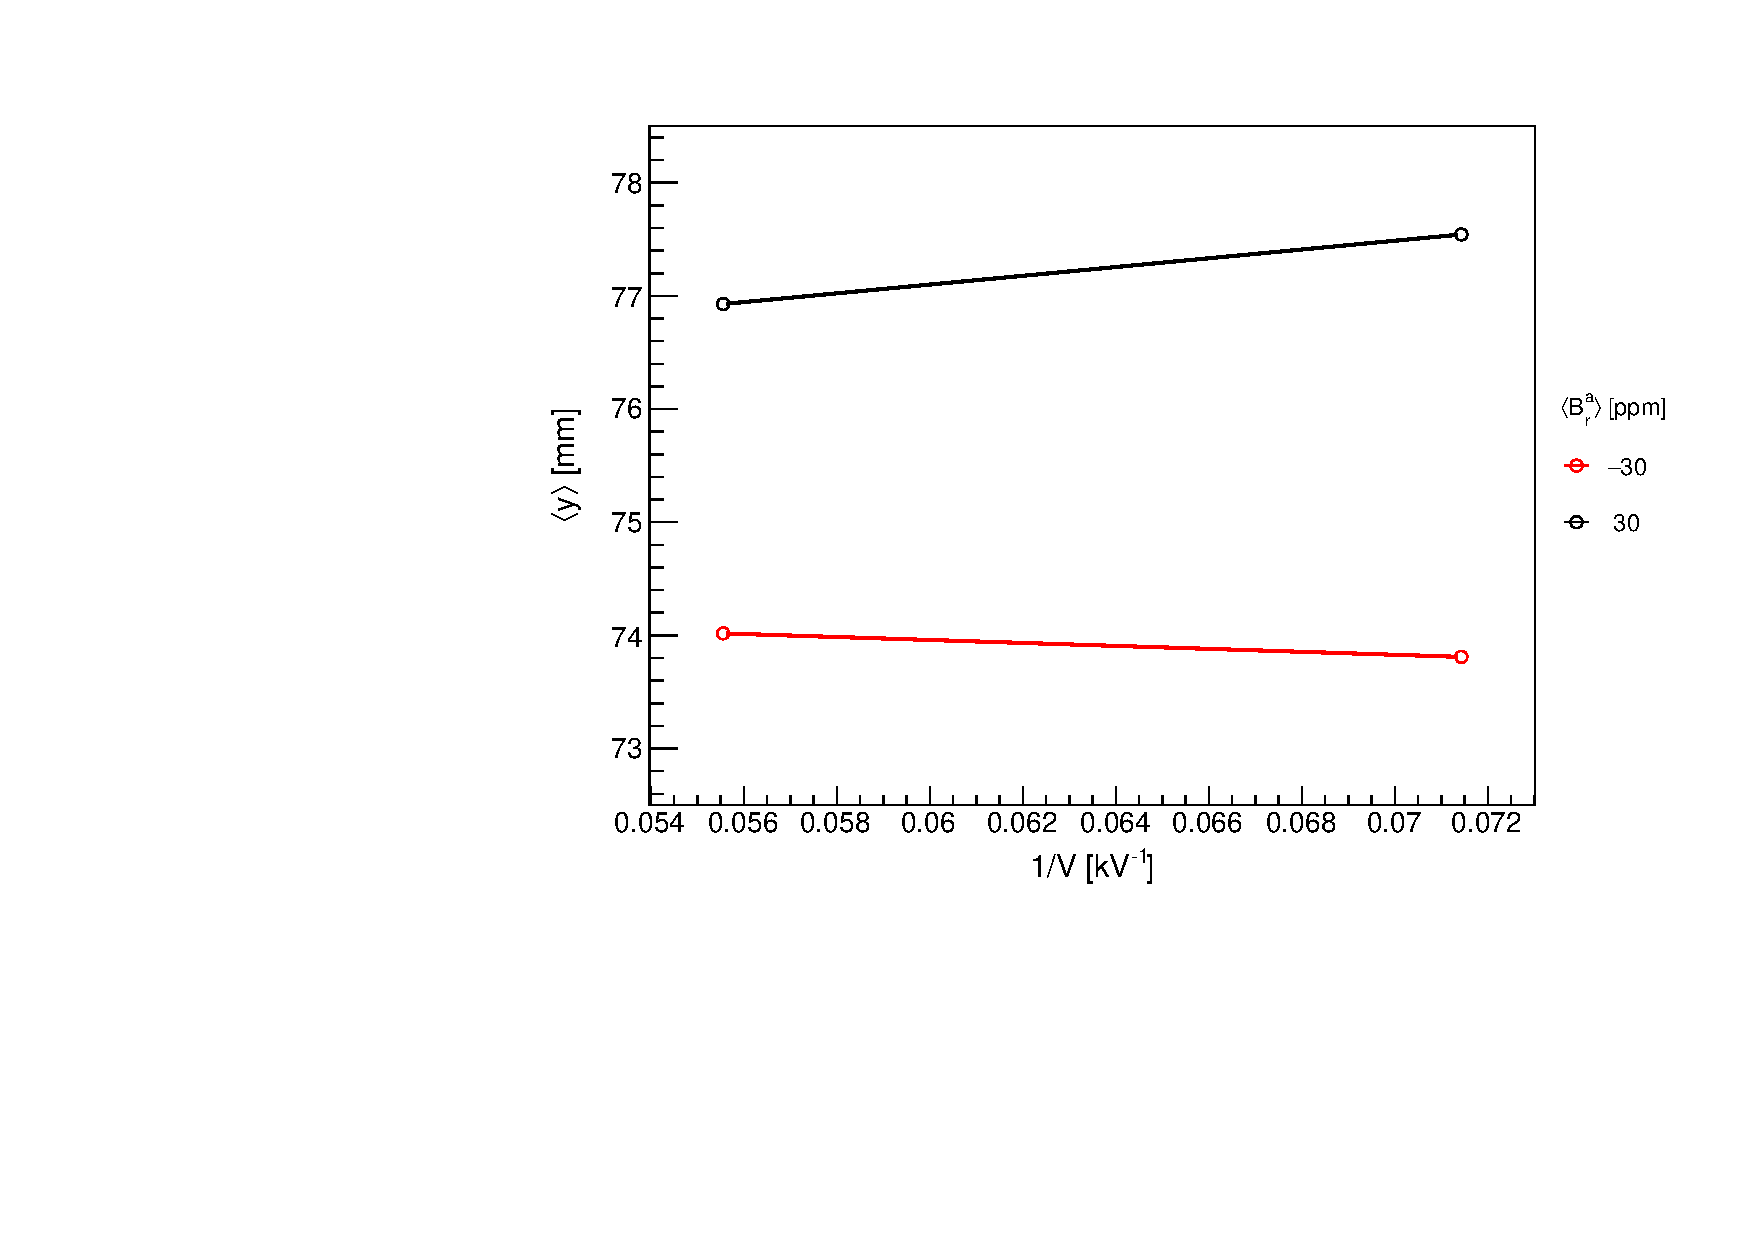
\includegraphics[trim={0 0 0 0},clip,width=0.49\textwidth]{Images/Chapter4/PreliminaryQuadScans.pdf}\label{subfig:PreliminaryQuadScans} }%\hfill
\subfloat[Preliminary $\langle B_{r}^{b} \rangle$ fit.]{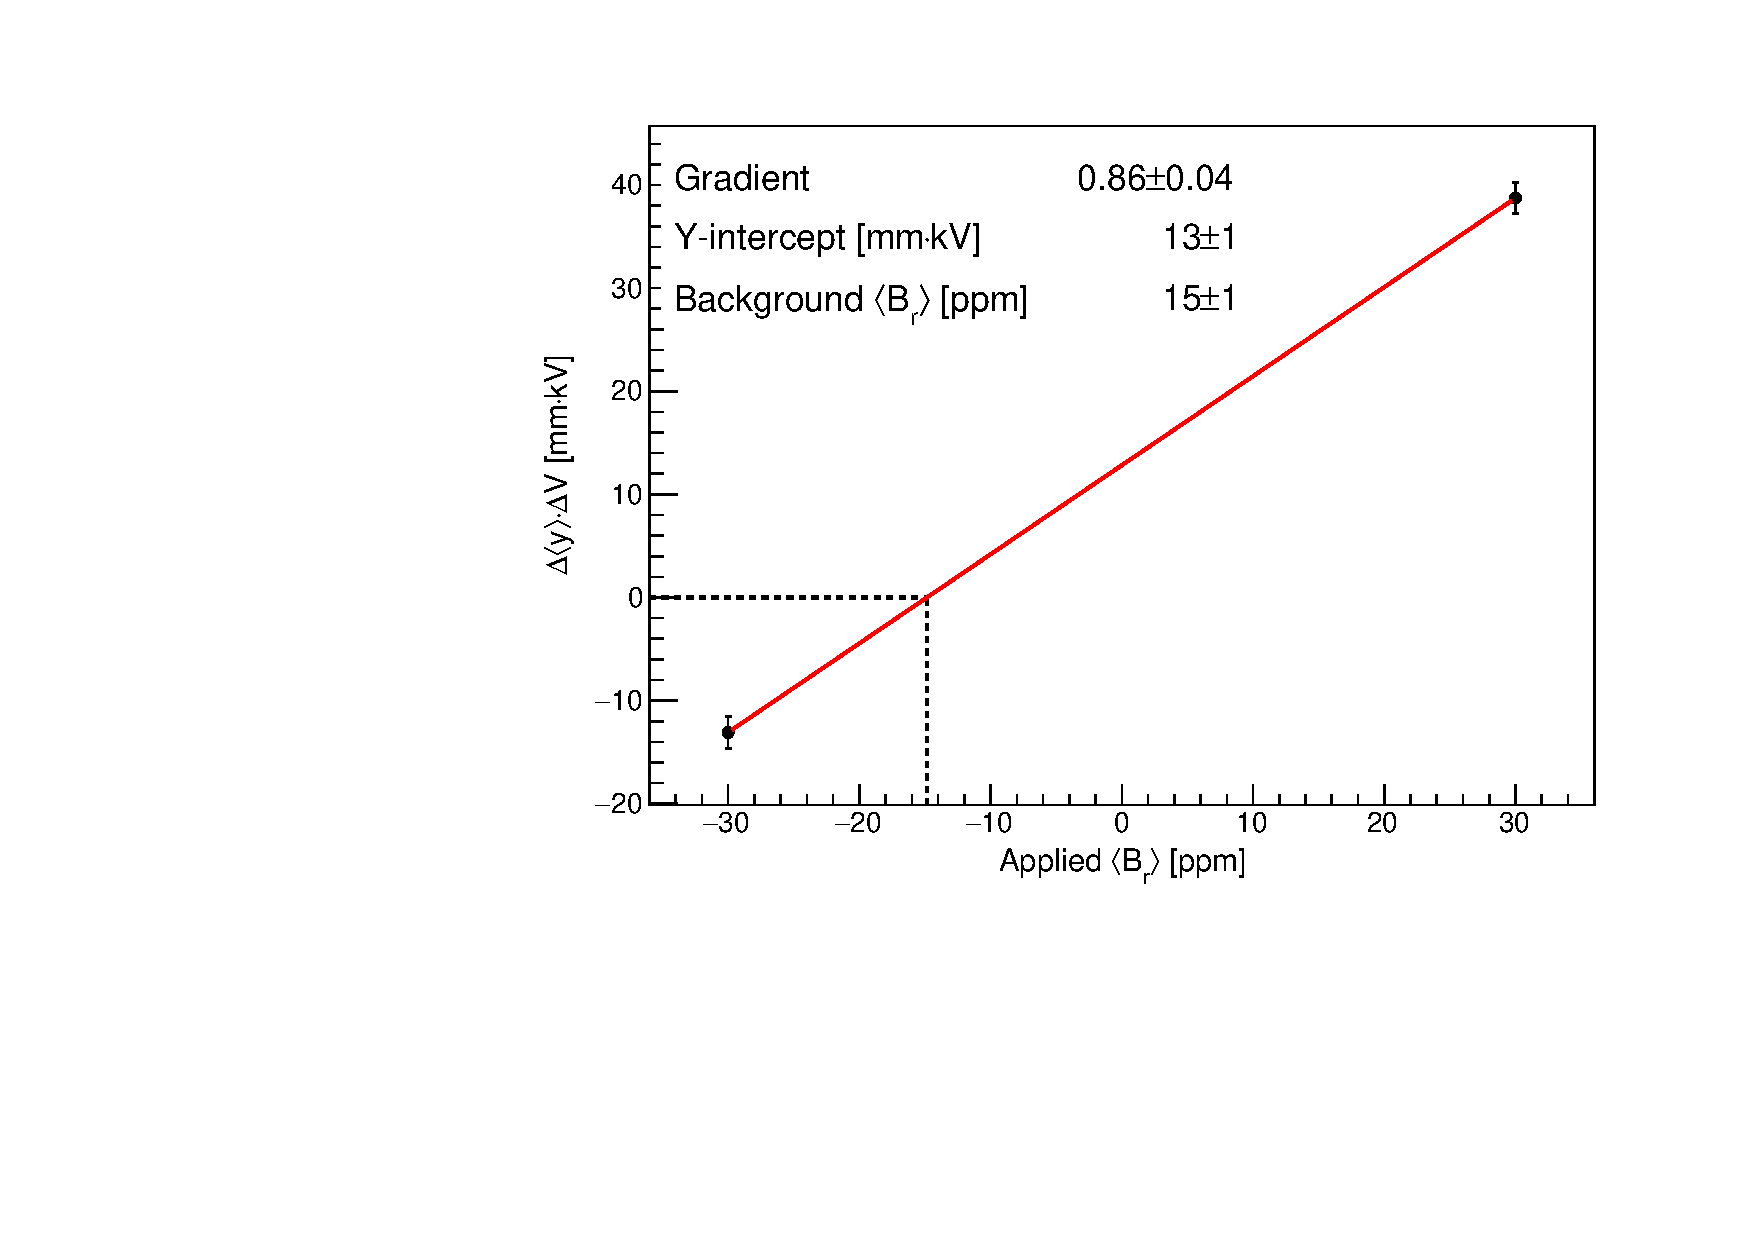
\includegraphics[trim={0 0 0 0},clip,width=0.49\textwidth]{Images/Chapter4/PreliminaryFieldFit.pdf}\label{subfig:PreliminaryFieldFit} }
\caption{The results of the preliminary measurement of $\langle B_{r}^{b} \rangle$ in Run-4, showing: (a) ESQ scans of $\langle y \rangle$ over $1/V$ for two SCC $\langle B_{r}^{a} \rangle$ set-points; (b) $\Delta \langle y \rangle \cdot \Delta V$ over $\langle B_{r}^{a} \rangle$. $\langle B_{r}^{b} \rangle$ was measured to be $15\pm1$ ppm.}
\label{fig:PreliminaryFits}
\end{figure}

\subsection{Primary results for the background radial field} 
%
Following the preliminary measurement, and subsequent zeroing of the background radial field, the beam intensity was increased to nominal and a second measurement was carried out on the \nth{30} of December 2020, using the full configuration described in Section \ref{sec:PlanningBr}. As planned, data was collected for $\sim20$ minutes (aiming for $\sim$4 million CTAGs) per set-point, targeting a precision of $\sim0.4$ ppm. Two settings, 18 kV at 10 ppm and 14 kV at $-50$ ppm, are not included in the analysis due to errors when loading those configurations in the field DAQ \cite{PrimaryMeasurementElog}. The results of the primary measurement are illustrated in Figure \ref{fig:PrimaryFits}, where the $\langle B_{r}^{b} \rangle$ was measured to be %From this measurement, $\$ results of this measurement was that the background radial field was found to be 
%
\begin{align*}
  \langle B_{r}^{b} \rangle = -0.4\pm0.6\text{ ppm},
\end{align*}
%
which is consistent with zero as expected, and has a statistical uncertainty of $<1$ ppm, as required.
%
\begin{figure}[t!]
\centering{}
\subfloat[Primary ESQ/SCC scans.]{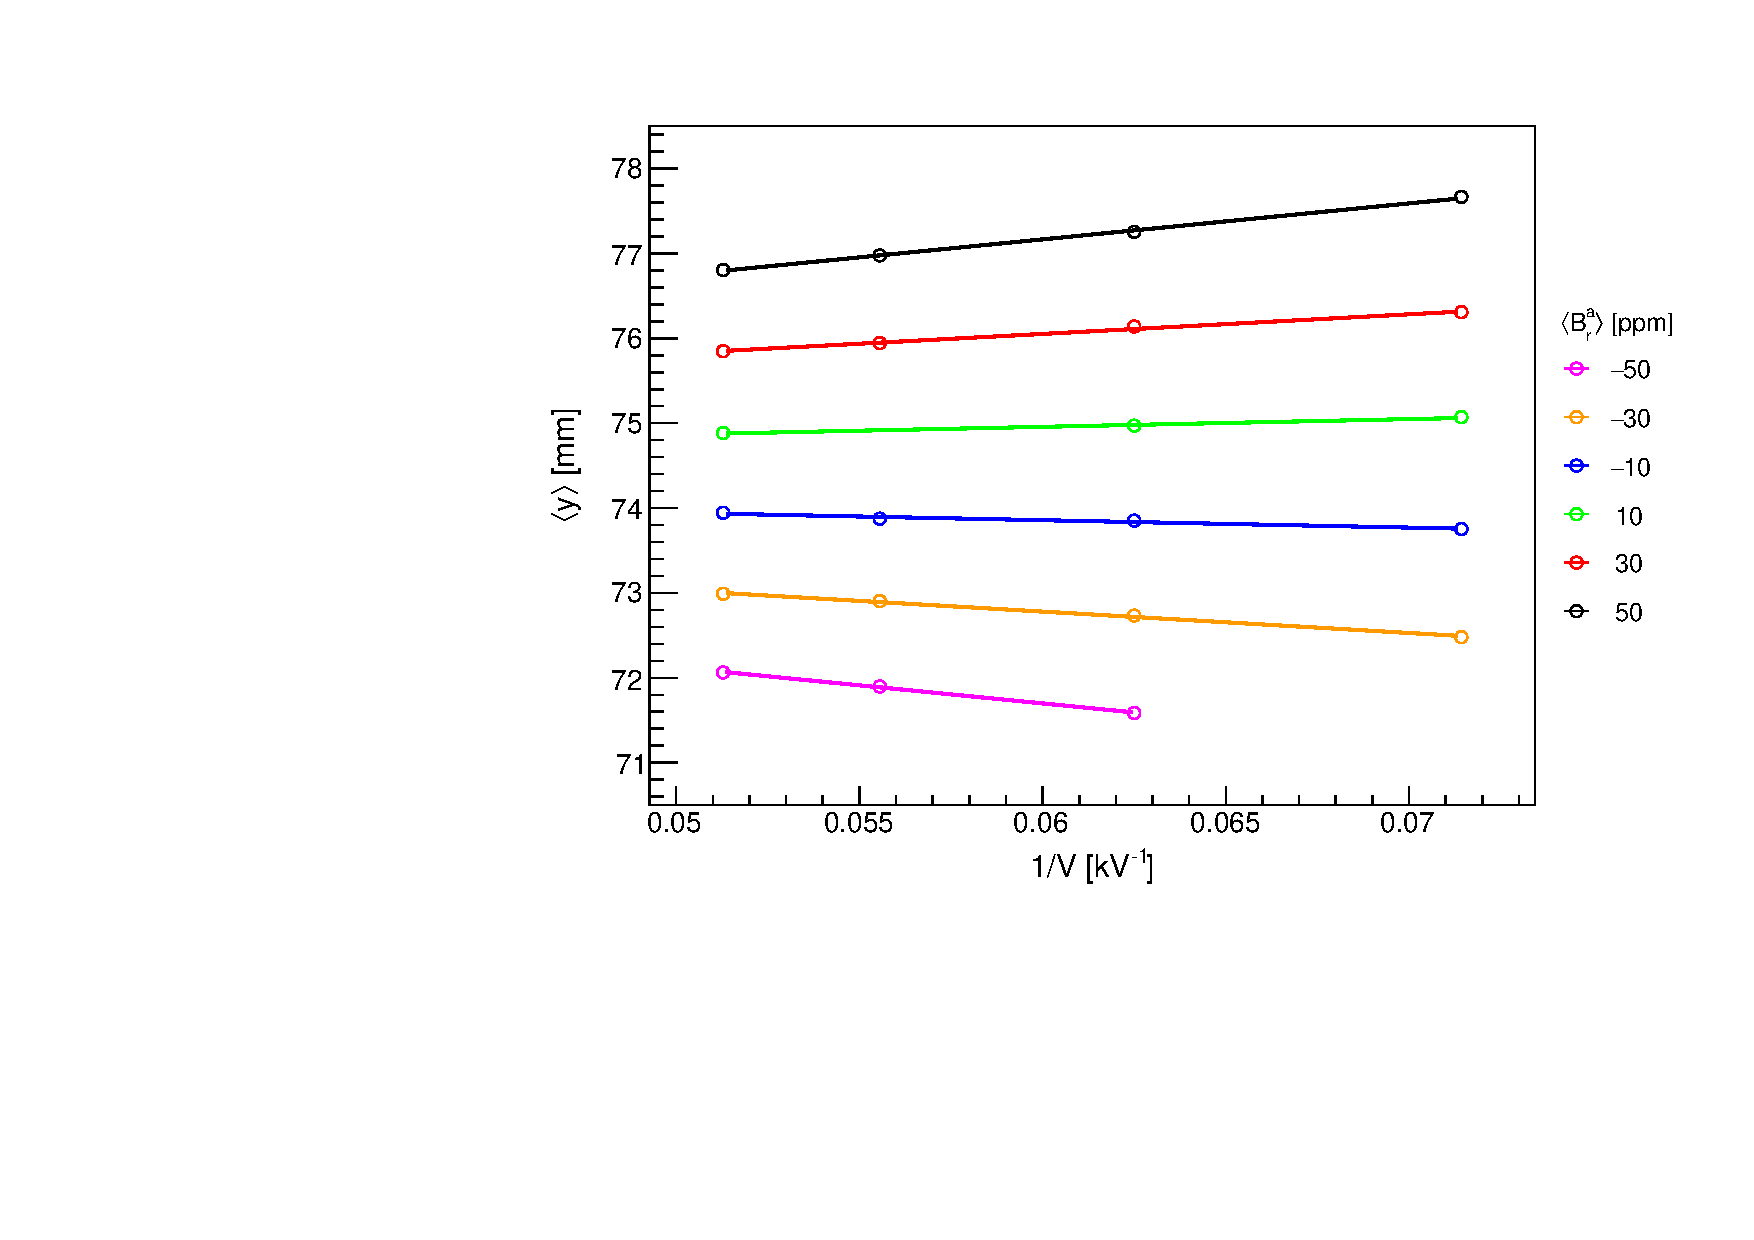
\includegraphics[trim={0 0 0 0},clip,width=0.49\textwidth]{Images/Chapter4/PrimaryQuadScans.pdf}\label{subfig:PrimaryQuadScans} }%\hfill
\subfloat[Primary $\langle B_{r}^{b} \rangle$ fit.]{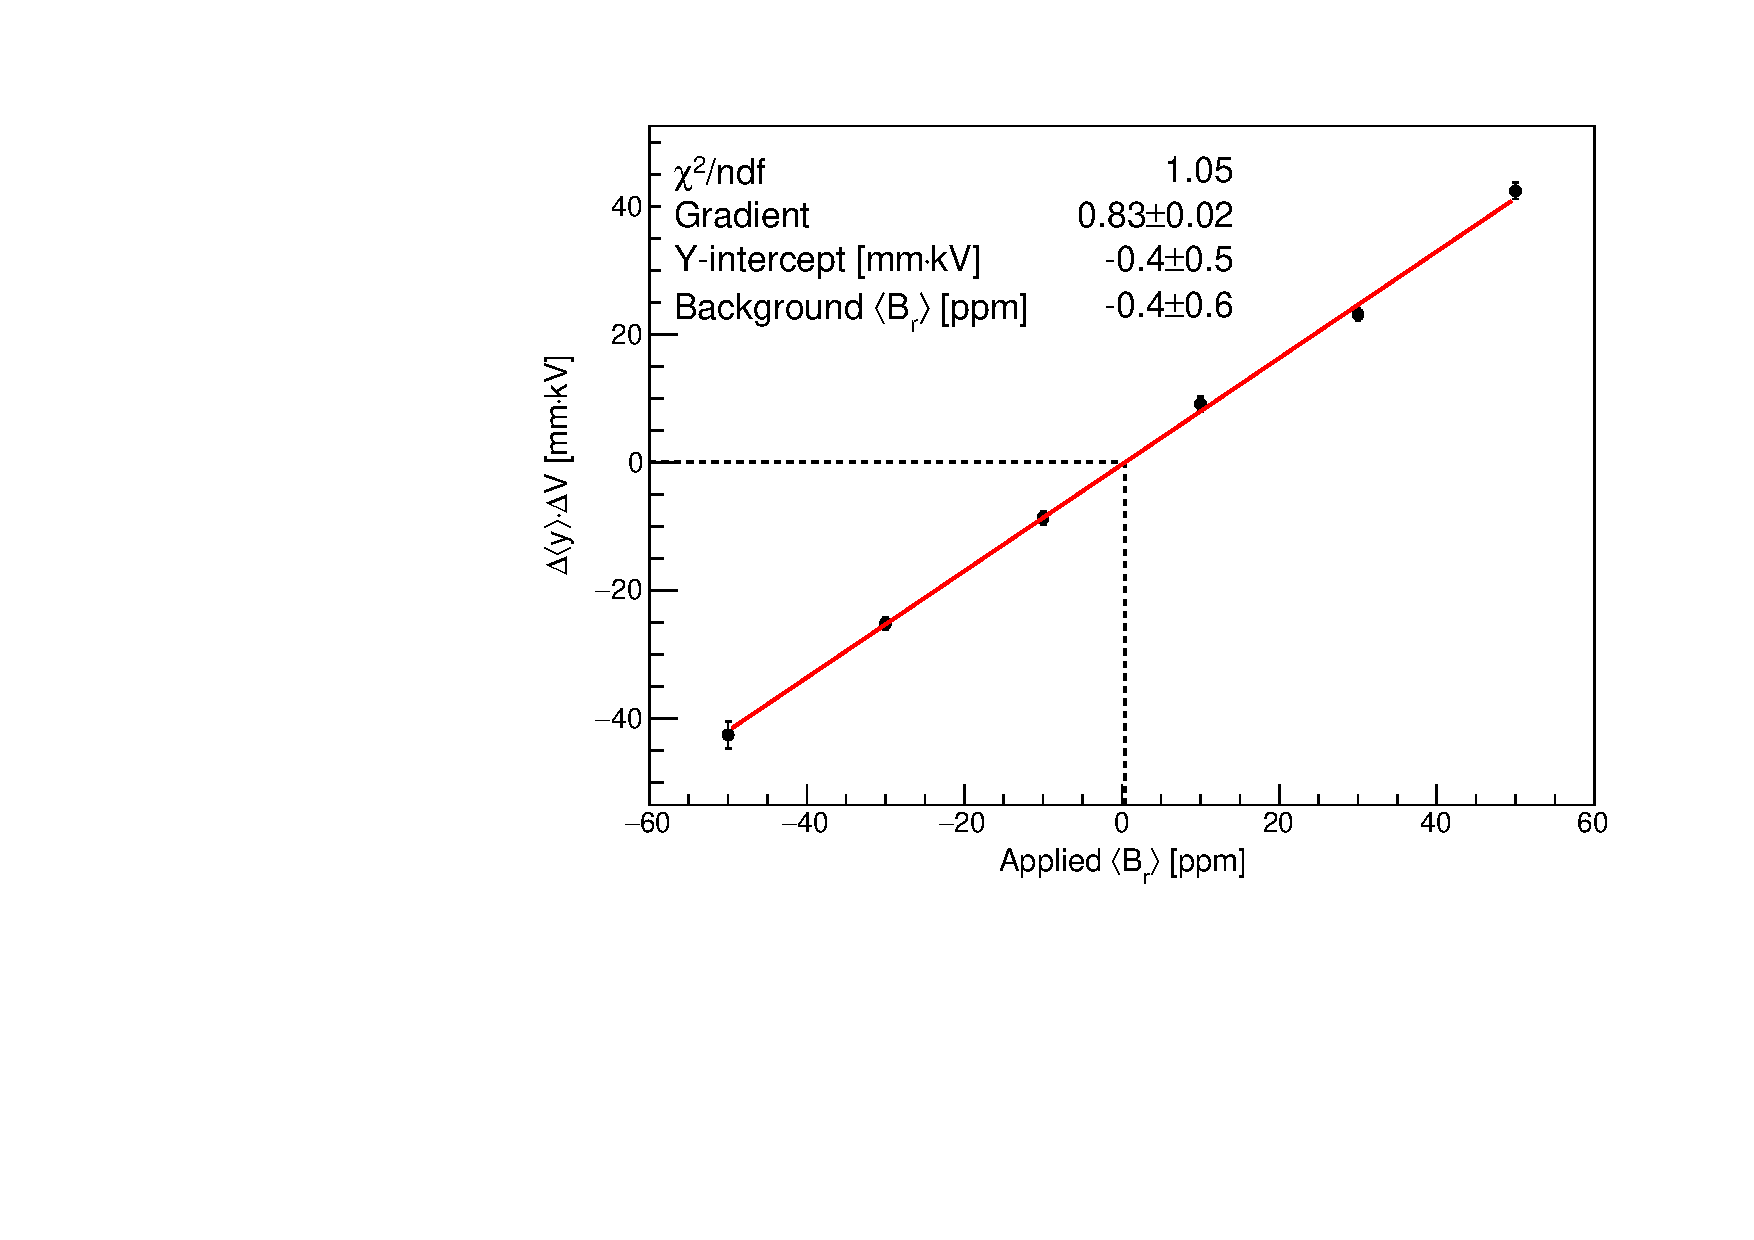
\includegraphics[trim={0 0 0 0},clip,width=0.49\textwidth]{Images/Chapter4/PrimaryFieldFit.pdf}\label{subfig:PrimaryFieldFit} }
\caption{The results of the primary measurement of $\langle B_{r}^{b} \rangle$ in Run-4, showing: (a) ESQ scans of $\langle y \rangle$ over $1/V$ for the full range of SCC $\langle B_{r}^{a} \rangle$ set-points; (b) $\Delta \langle y \rangle \cdot \Delta V$ over $\langle B_{r}^{a} \rangle$. $\langle B_{r}^{b} \rangle$ was measured to be $-0.4\pm0.6$ ppm.}
\label{fig:PrimaryFits}
\end{figure}

\subsection{Analysis cuts}

The quantity being directly observed throughout these measurements was the ring average vertical cluster position, $\langle y \rangle$, which depends on the energy and in-fill hit times of the decay positrons. Cuts were implemented to select a region of parameter space where $\langle y \rangle$ is stable, illustrated in Figure \ref{fig:Cuts}, with the red lines outlining the following regions used in the analysis:
%
\begin{align*}
23 < t \text{ [$\mu$s]} < 300 \quad \text{and} \quad 1000 < E \text{ [MeV]} < 2750.
\end{align*}
%
The possible factors driving these regions of instability are: ESQ charging at early times, a low muon population at late times, positron pileup at high energies, and lost muons at low energies. 

\begin{figure}[t!]
\centering{}
\subfloat[Cluster energy against time in-fill.]{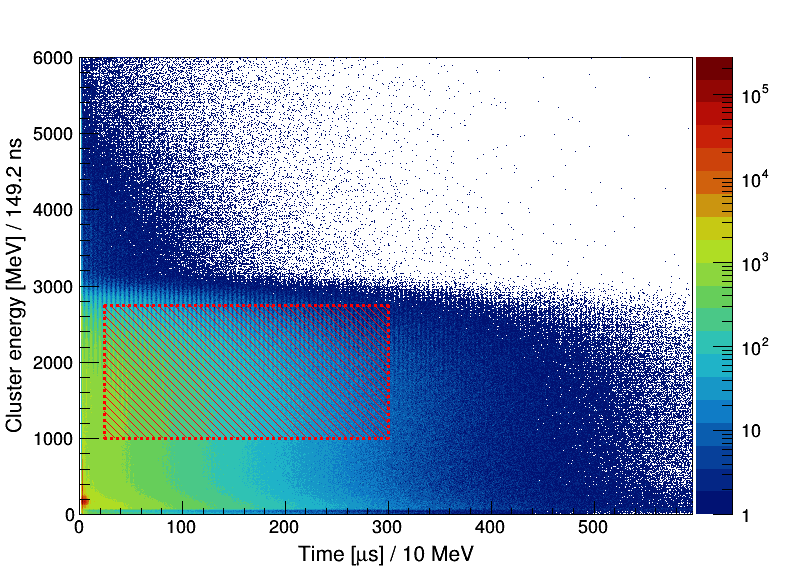
\includegraphics[trim={0 0 0 0},clip,width=0.49\textwidth]{Images/Chapter4/cluTE_cuts.png}\label{subfig:2DCuts} }\hfill
\subfloat[$\langle y \rangle$ against cluster energy.]{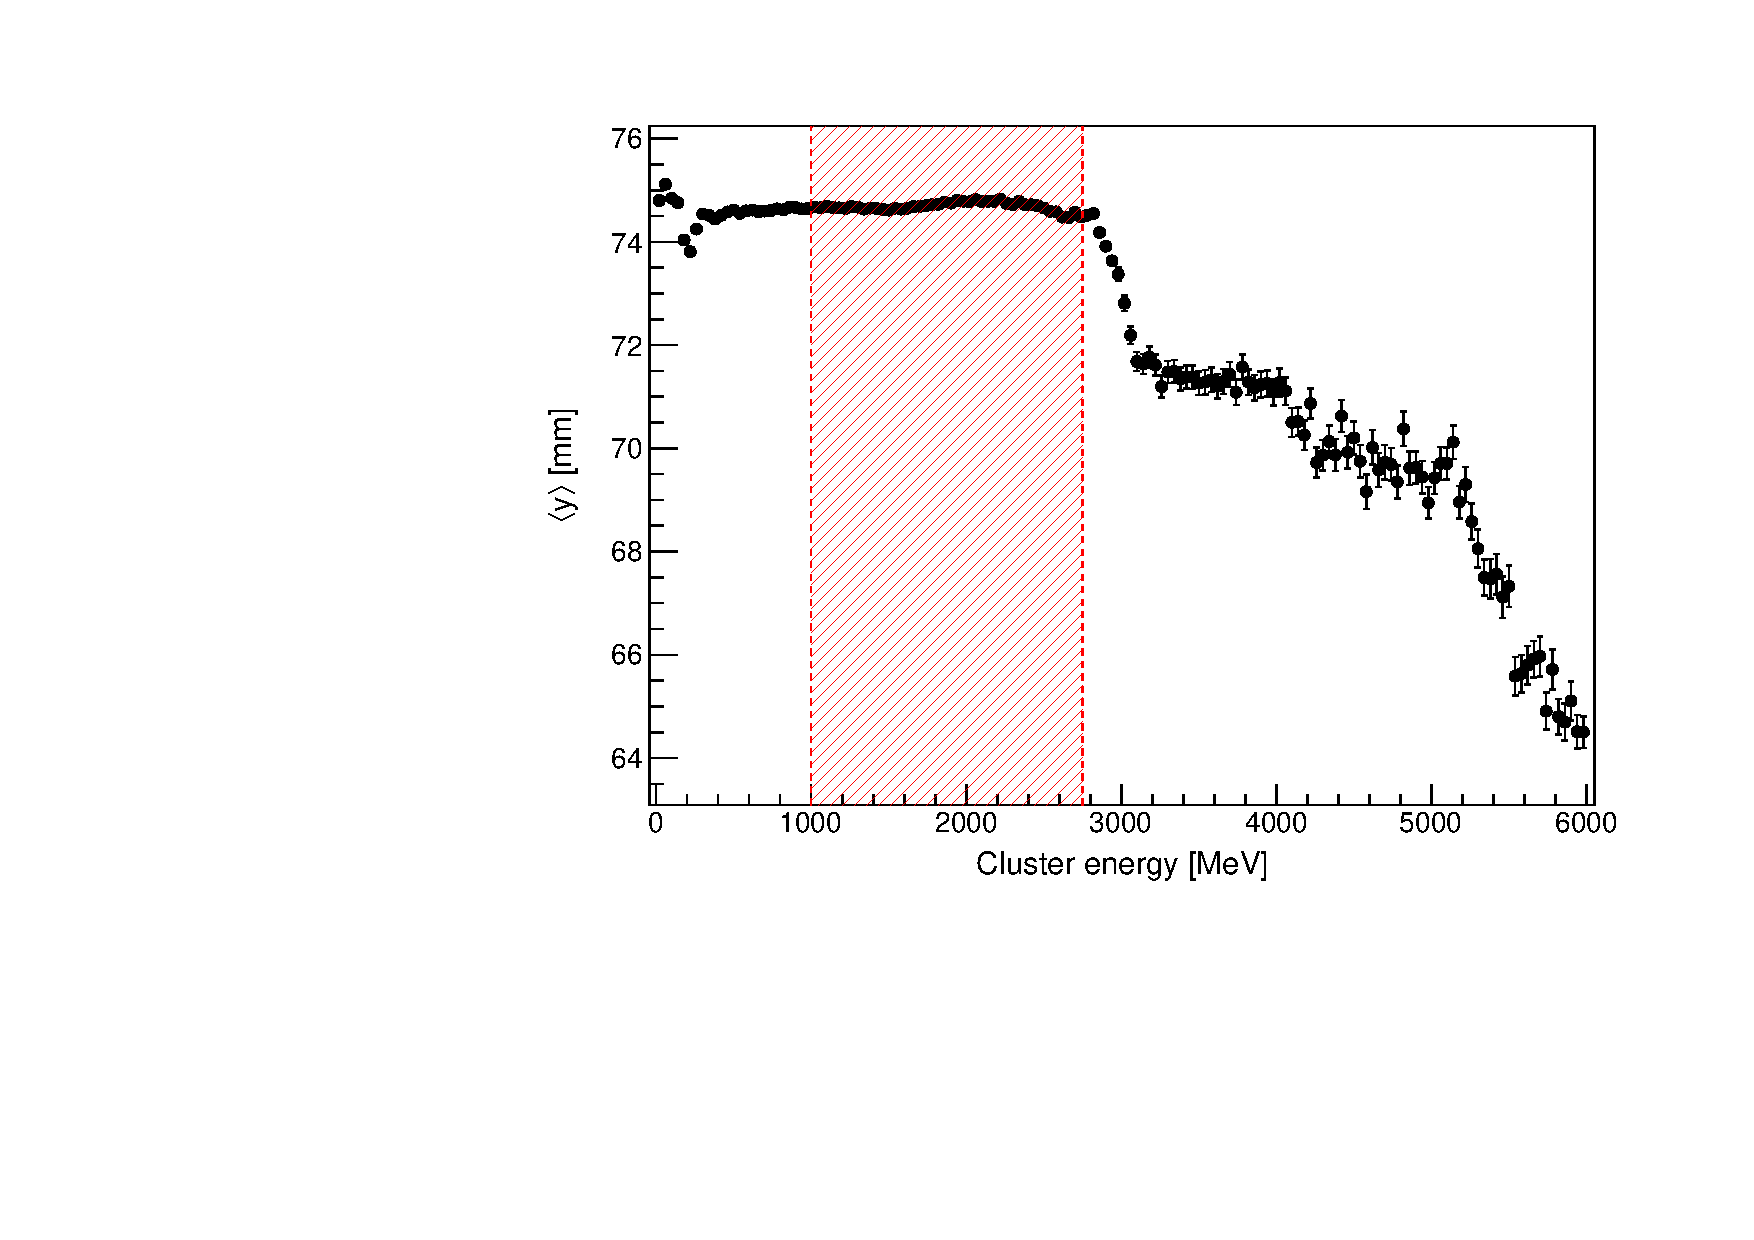
\includegraphics[trim={0 0 0 0},clip,width=0.49\textwidth]{Images/Chapter4/cluEY_px.pdf}\label{subfig:EnergyCuts} }%\hfill
\subfloat[$\langle y \rangle$ against time in-fill.]{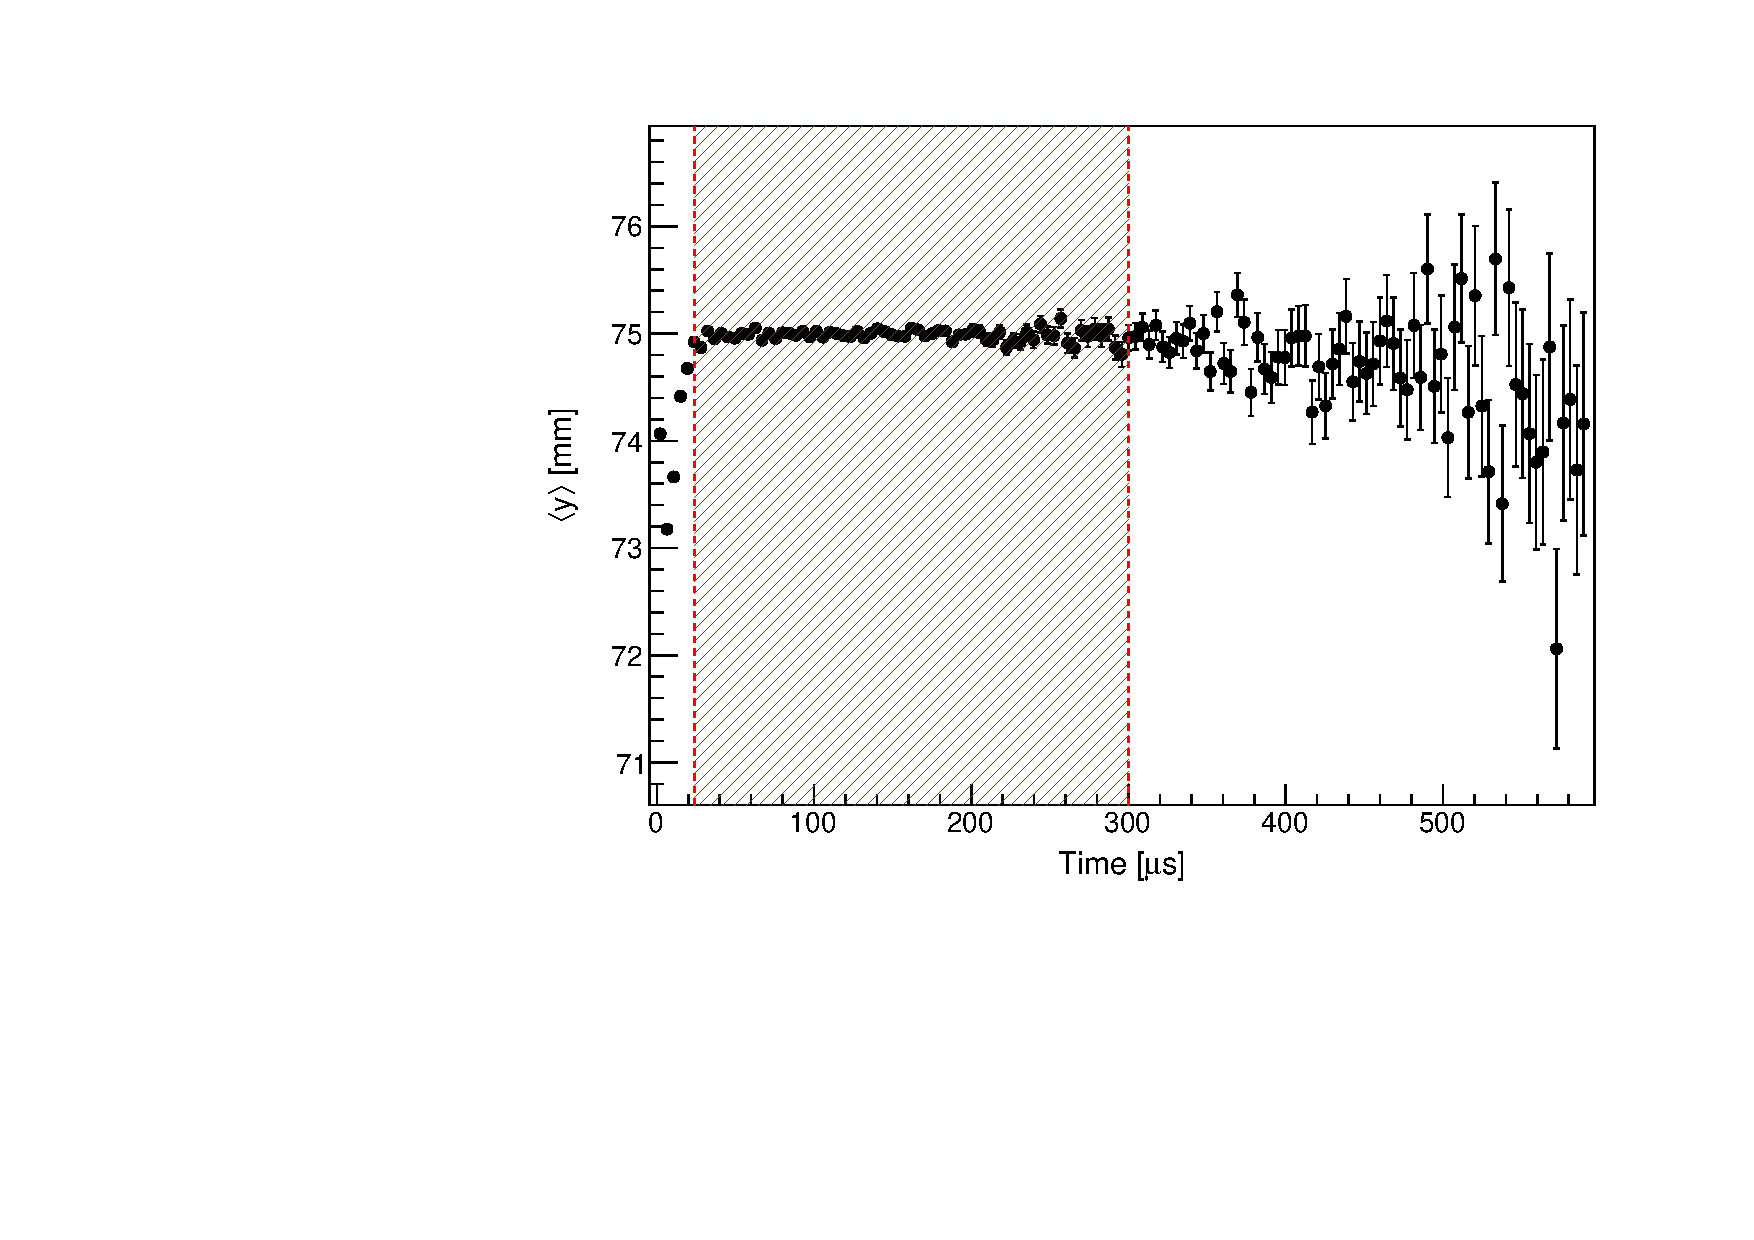
\includegraphics[trim={0 0 0 0},clip,width=0.49\textwidth]{Images/Chapter4/cluTY_px.pdf}\label{subfig:TimeCuts} }
\caption{Cuts in time and energy used during the analysis of $\langle B_{r}^{b} \rangle$, optimised for stability in $\langle y \rangle$.}
\label{fig:Cuts}
\end{figure}

\subsection{Extrapolation results}\label{subsection:ExtrapolatingTheRadialField}

\begin{figure}[t!]
\centering{}
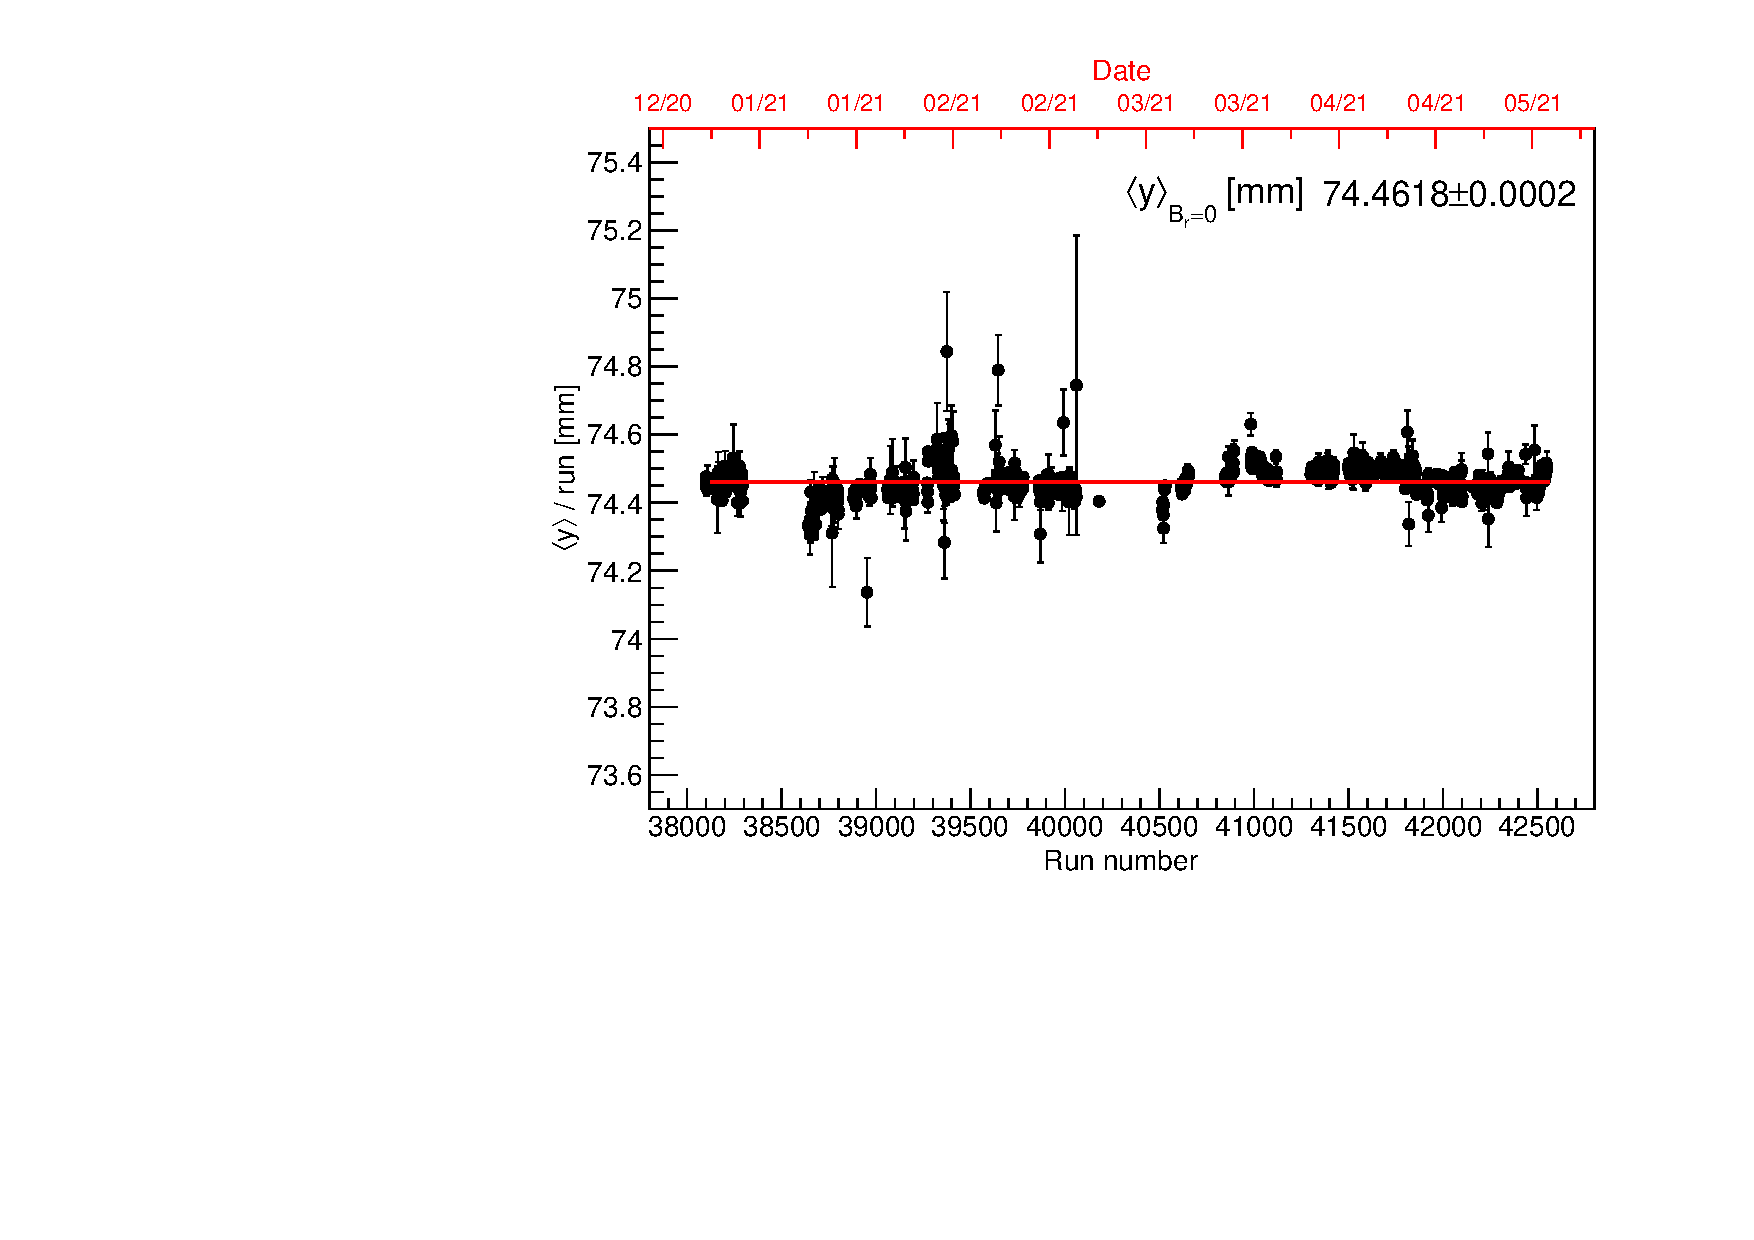
\includegraphics[trim={0 0 0 0},clip,width=0.65\textwidth]{Images/Chapter4/Fit_NoBadCalos_Run4_2021.pdf}
\caption{A zeroth order fit to $\langle y \rangle$ over a period of Run-4 where $\langle B_{r} \rangle$ was known to be zero. The result is an uncertainty weighted average which may be used as a reference position, $\langle y \rangle_{\text{ref}}$, to estimate $\langle B_{r} \rangle$ in any E989 dataset.}
\label{fig:RefPos}
\end{figure} 
%
\begin{figure}[t!]
\centering{}
\subfloat[]{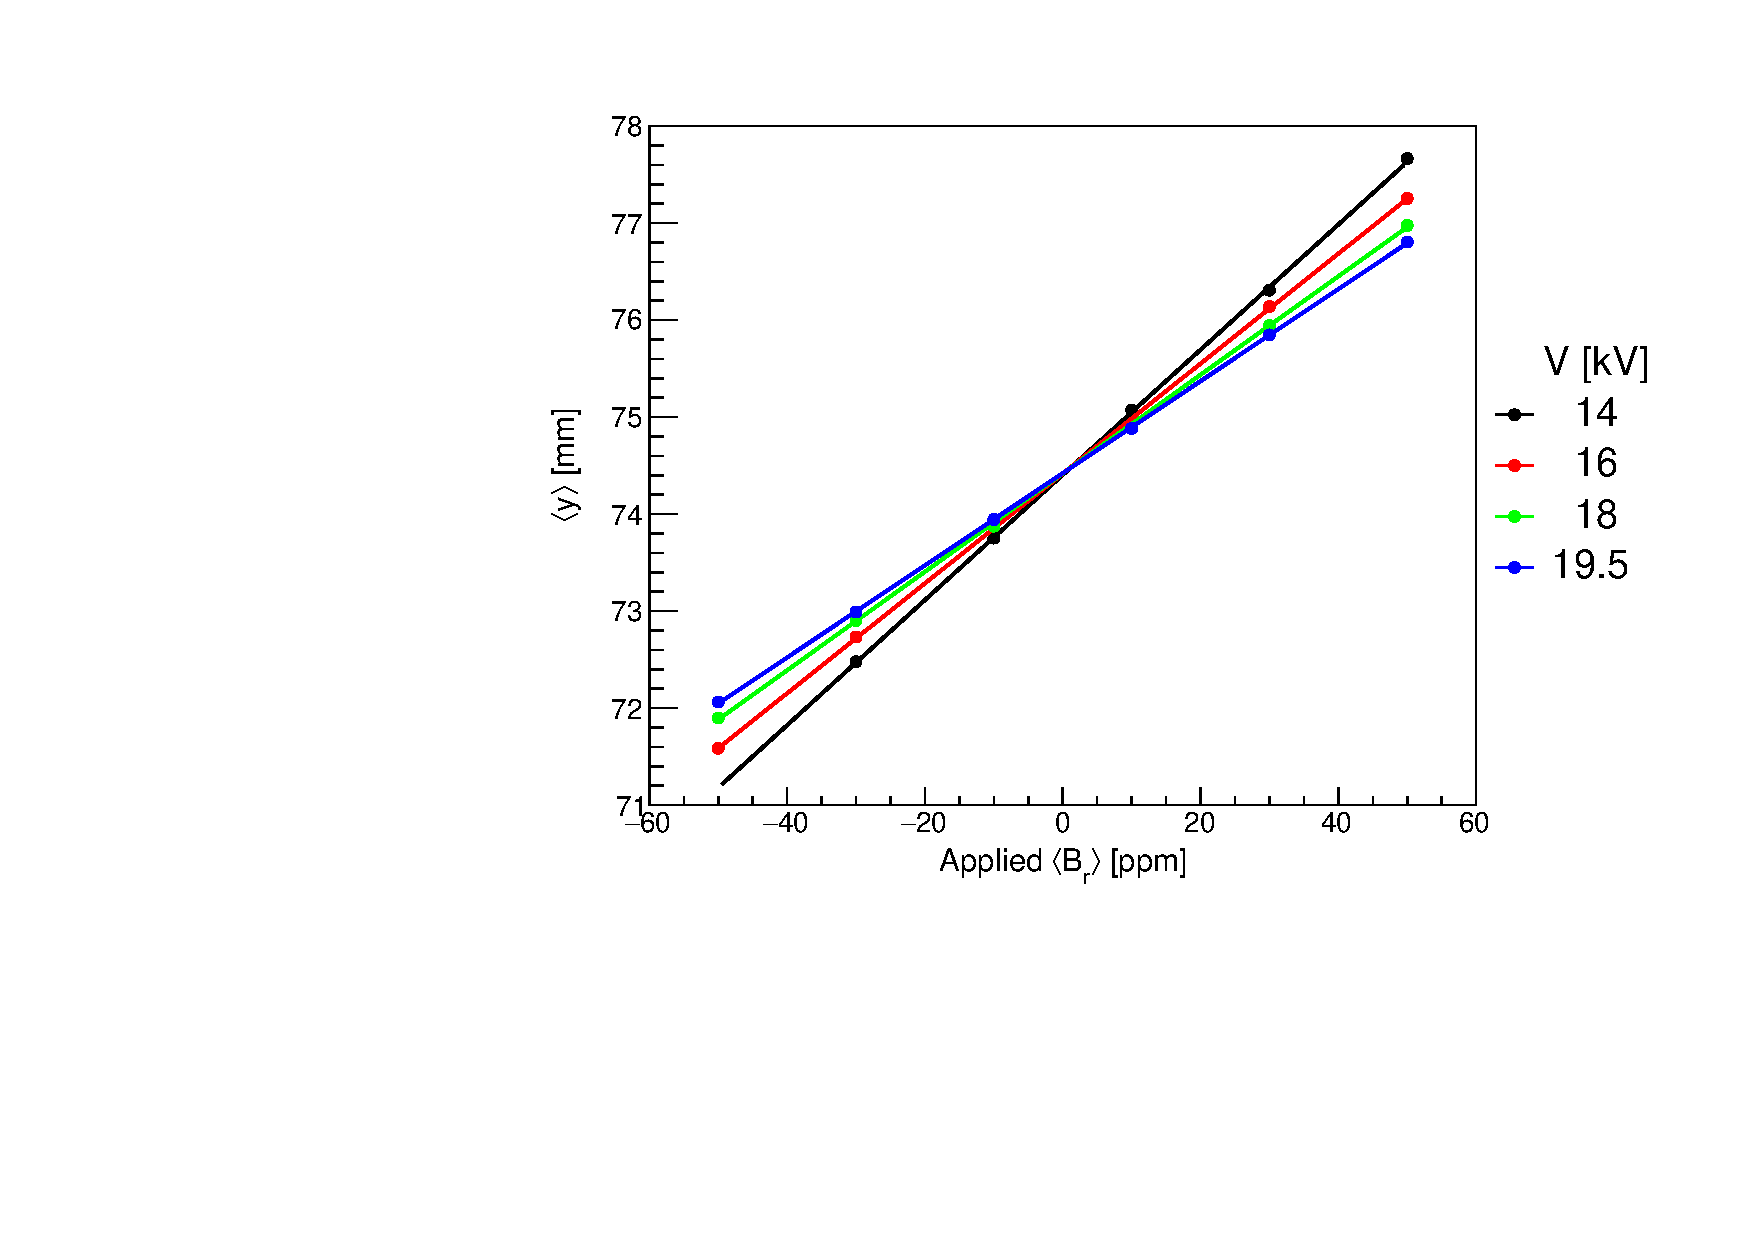
\includegraphics[trim={0 0 0 0},clip,width=0.49\textwidth]{Images/Chapter4/InverseQuadFits.pdf} }%\hfill
\subfloat[]{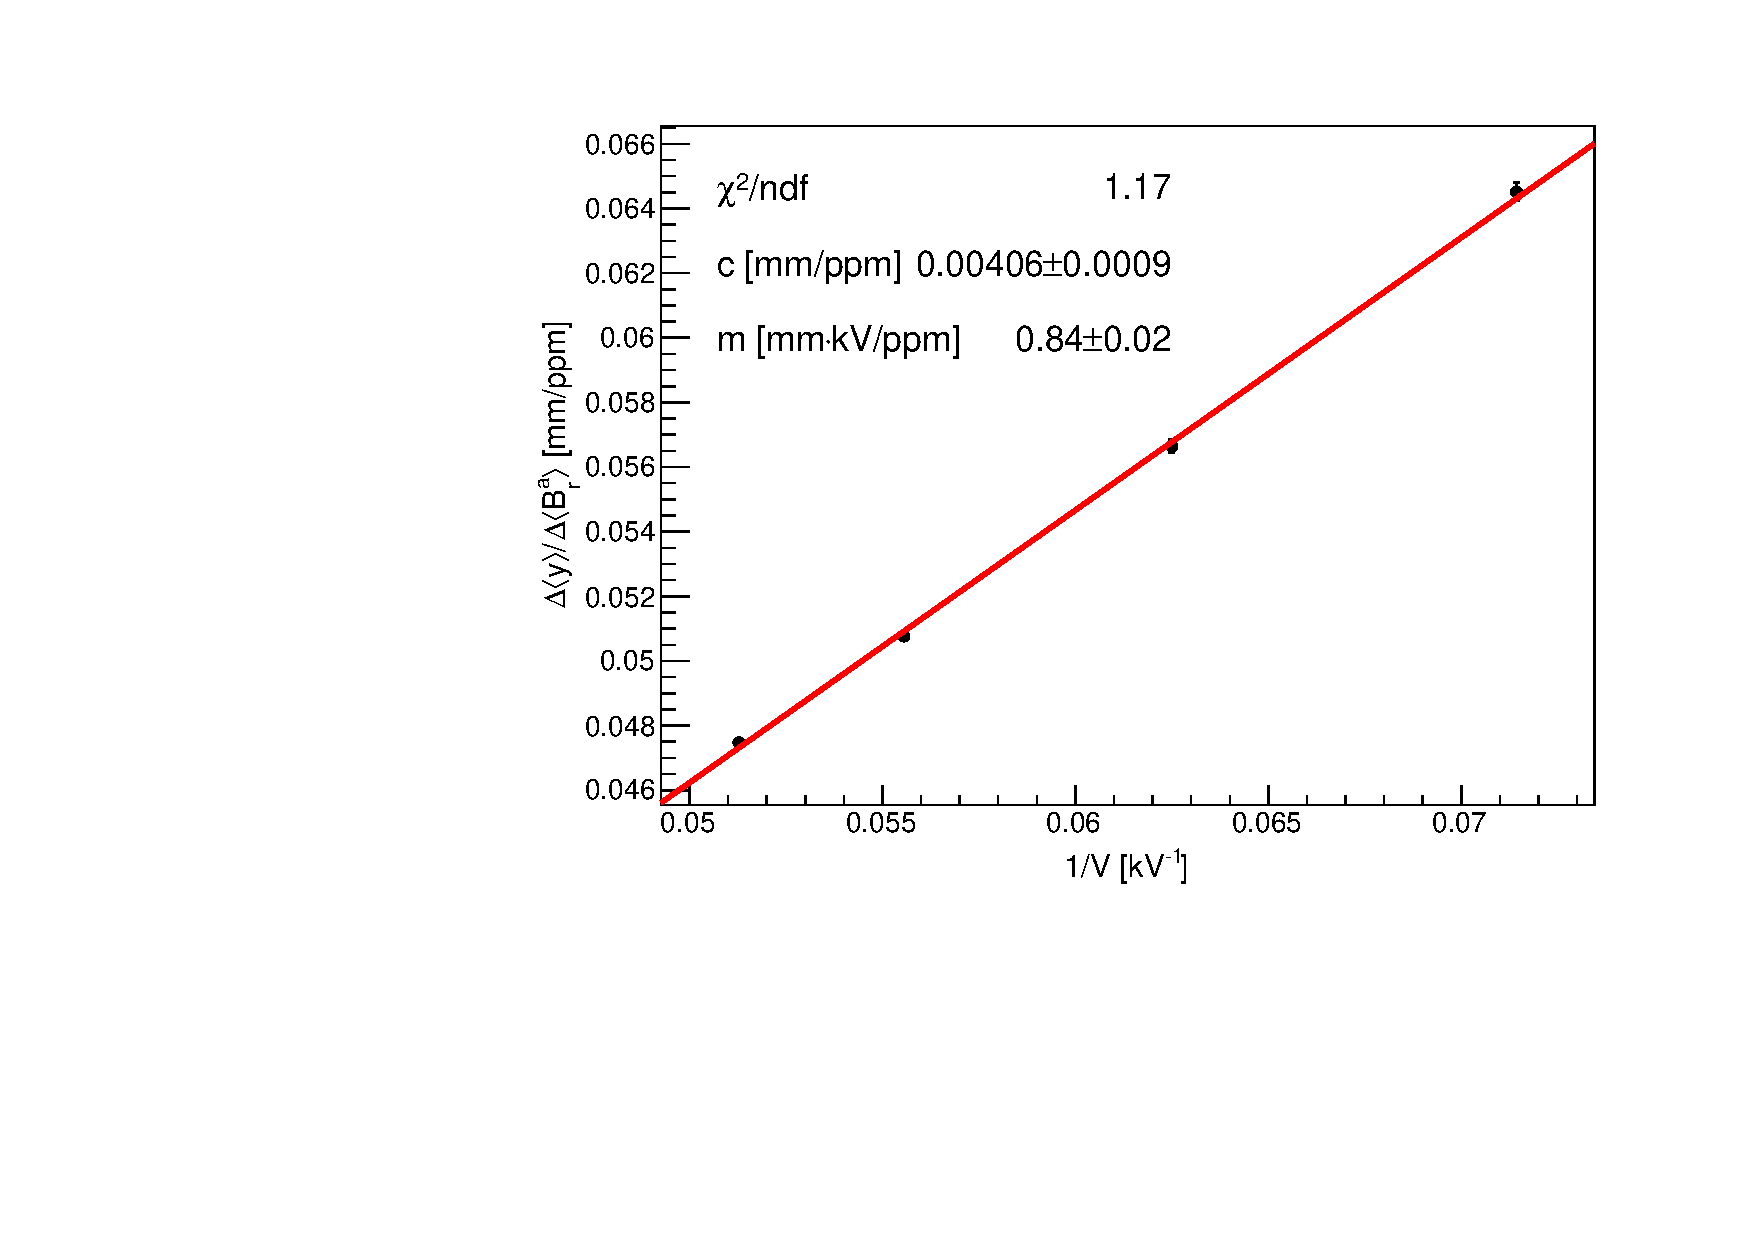
\includegraphics[trim={0 0 0 0},clip,width=0.49\textwidth]{Images/Chapter4/mainFit_mm2ppm.pdf}}
\caption{Fits for the radial field conversion factor, $k$, showing: (a) fits to scans of $\langle y \rangle$ over $\langle B_{r}^{a} \rangle$; (b) a fit the gradients $\Delta \langle y \rangle / \Delta \langle B_{r}^{a} \rangle$ against $1/V$, giving a function which may be evaluated at the voltage used in the dataset of interest to obtain $k$.}
\label{fig:EmpiricalConversion}
\end{figure}

Following the measurements of $\langle B_{r}^{b} \rangle$, $\langle B_{r} \rangle$ was estimated for various datasets from Run-1 through to Run-5. The period of the runs selected to act as a reference position, $\langle y \rangle_{\text{ref}}$, follows the primary radial field measurement in Run-4, and consists of runs 38100-42588. This corresponds to a period between the \nth{5} of January 2021 and the \nth{10} of May 2021. The uncertainty weighted $\langle y \rangle$ was measured via a zeroth order polynomial fit over this period, as shown in Figure \ref{fig:RefPos}, giving 
%
\begin{align*}
  \langle y \rangle_{\text{ref}} = 74.4618\pm0.0002\text{ mm.}
\end{align*} 
% 
%
This done, the constant required to convert between $\Delta \langle y \rangle$ and $\Delta \langle B_{r} \rangle$, $k$, from Equation \ref{eqn:EmpricalConversionFactor}, was derived from the same data used in the primary measurement of $\langle B_{r}^{b} \rangle$. Fits for $k$ are shown in Figure \ref{fig:EmpiricalConversion}, giving
%
\begin{align*}
    k\,(18.3 \text{ kV}) = 19.9\pm0.6 \text{ ppm/mm} \\
    k\,(20.4 \text{ kV}) = 21.9\pm0.7 \text{ ppm/mm},
\end{align*}
%
where the ESQ voltage is 18.3 kV for all datasets except Run-1b and Run-1c, where it is 20.4 kV (as given in Table \ref{tbl:MeasPeriods}) \cite{BeamDynamics}.

\begin{figure}[b!]
\centering{}
\subfloat[Adjacent calorimeter $\Delta\langle y \rangle$.]{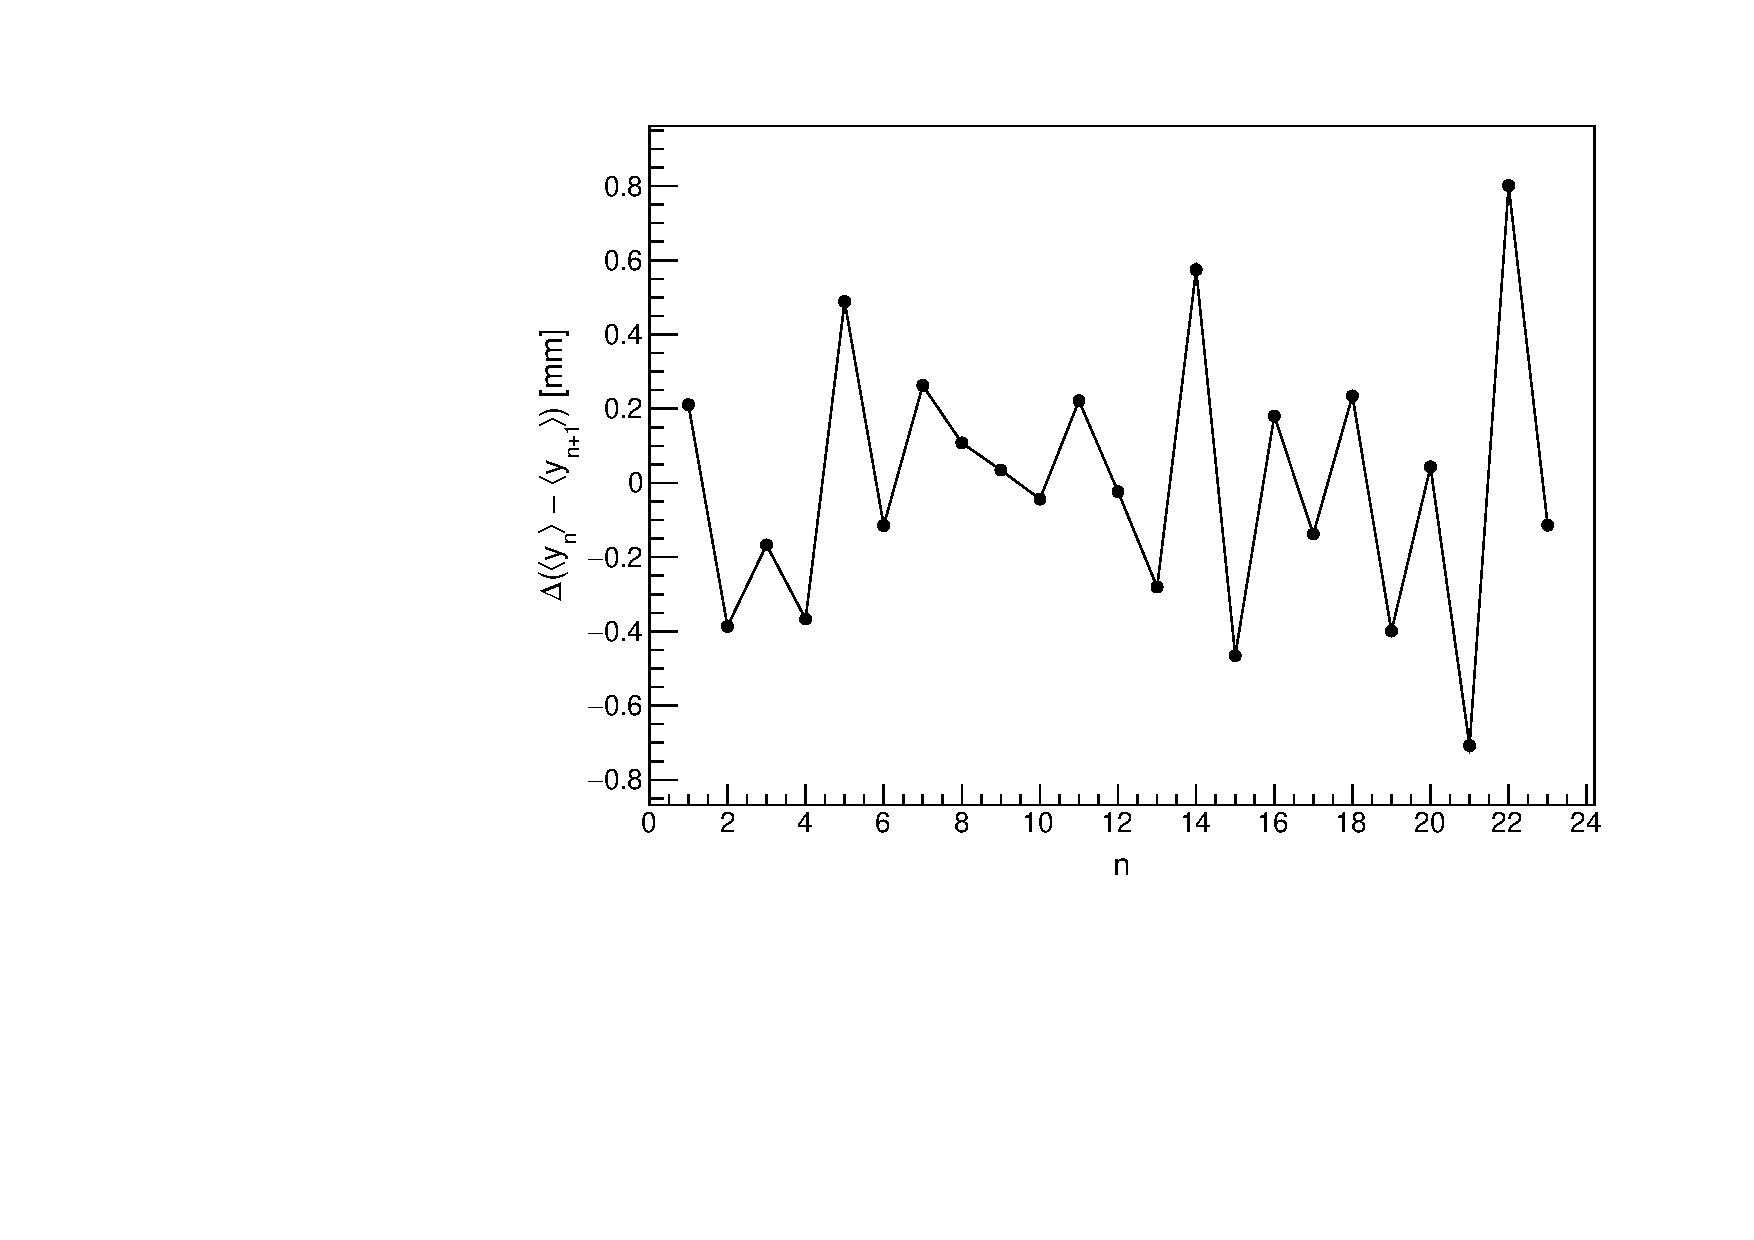
\includegraphics[trim={0 0 0 0},clip,width=0.49\textwidth]{Images/Chapter4/grDiff_gm2pro_daq_full_run1_60h_5039A_GLdocDB16021-v2.pdf}\label{subfig:grComp} } 
\subfloat[The change in adjacent calorimeter $\Delta\langle y \rangle$. ]{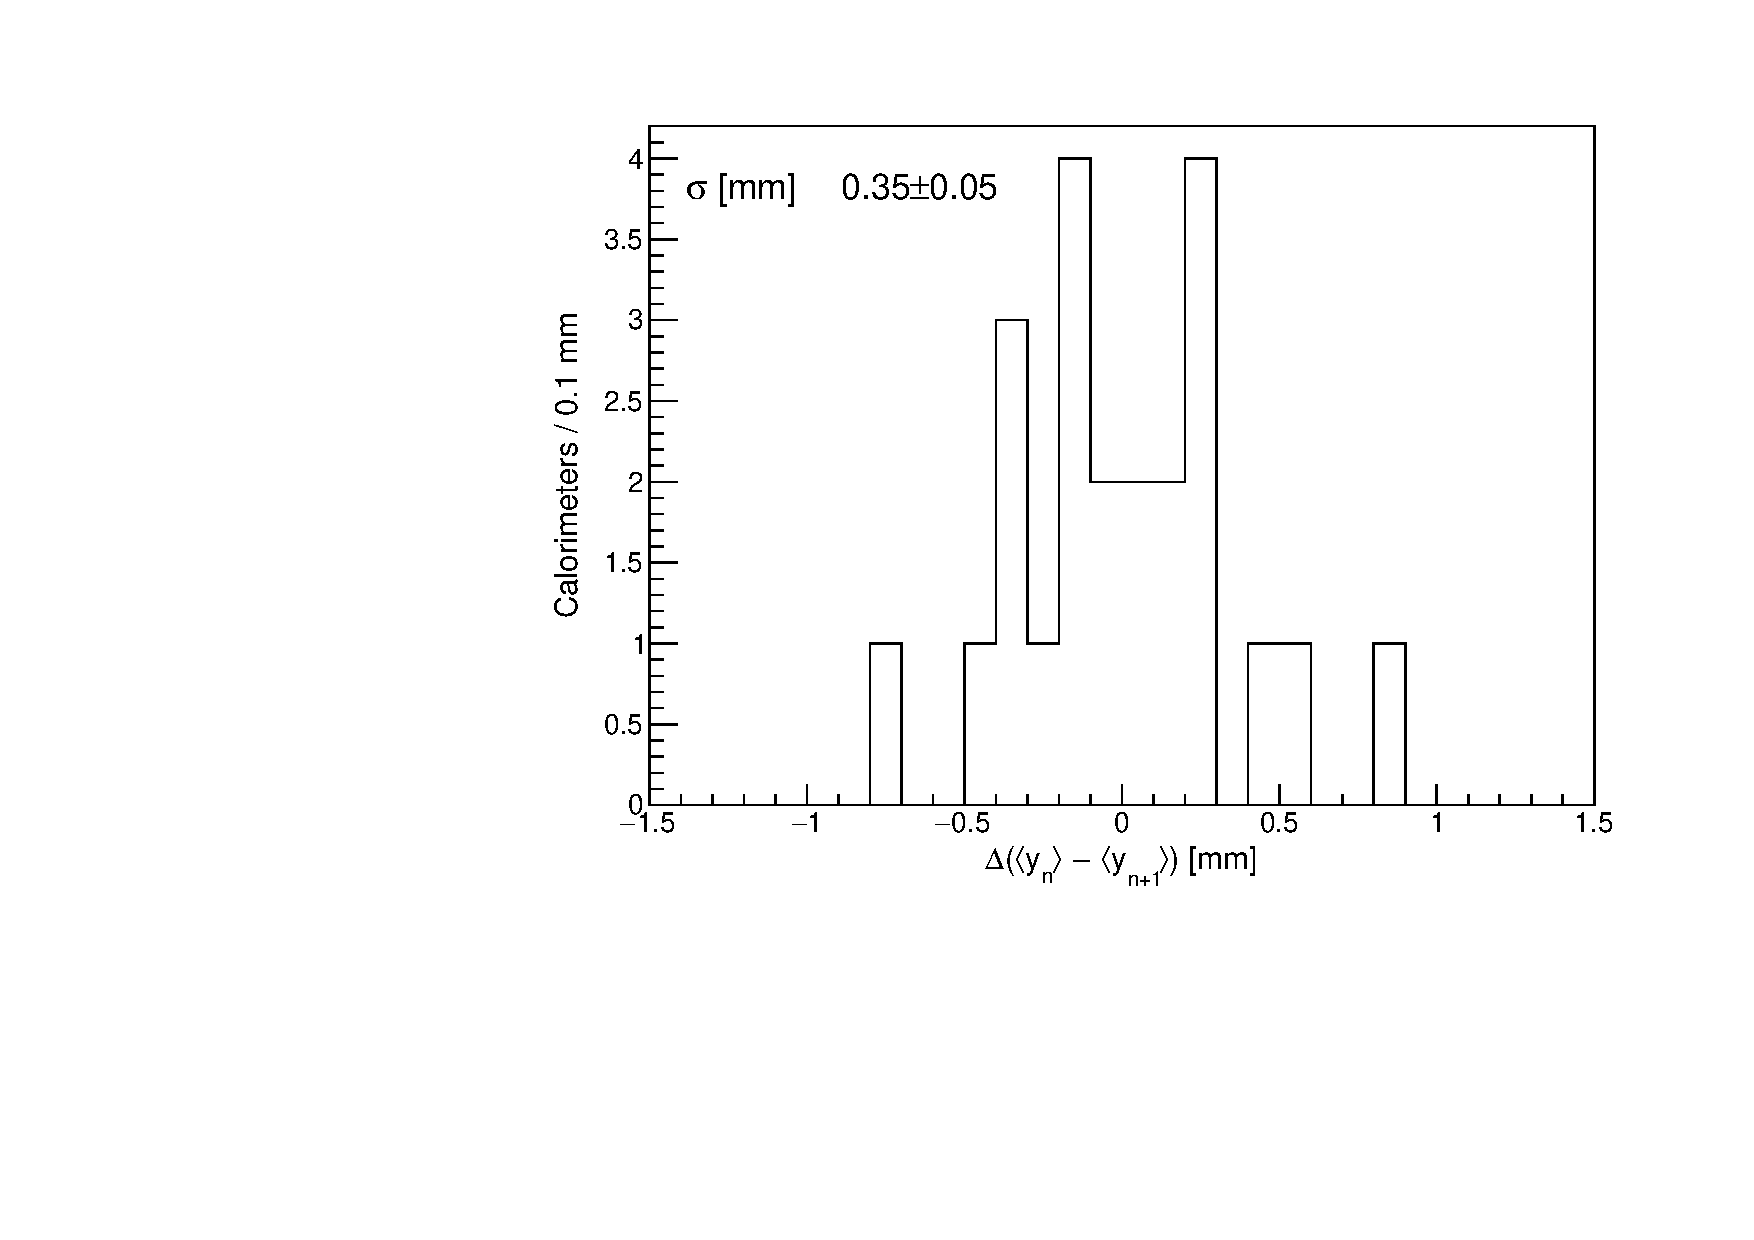
\includegraphics[trim={0 0 0 0},clip,width=0.49\textwidth]{Images/Chapter4/hDiff_gm2pro_daq_full_run1_60h_5039A_GLdocDB16021-v2.pdf}\label{subfig:hDiff} }\hfill
\subfloat[The drift in $\langle y \rangle$.]{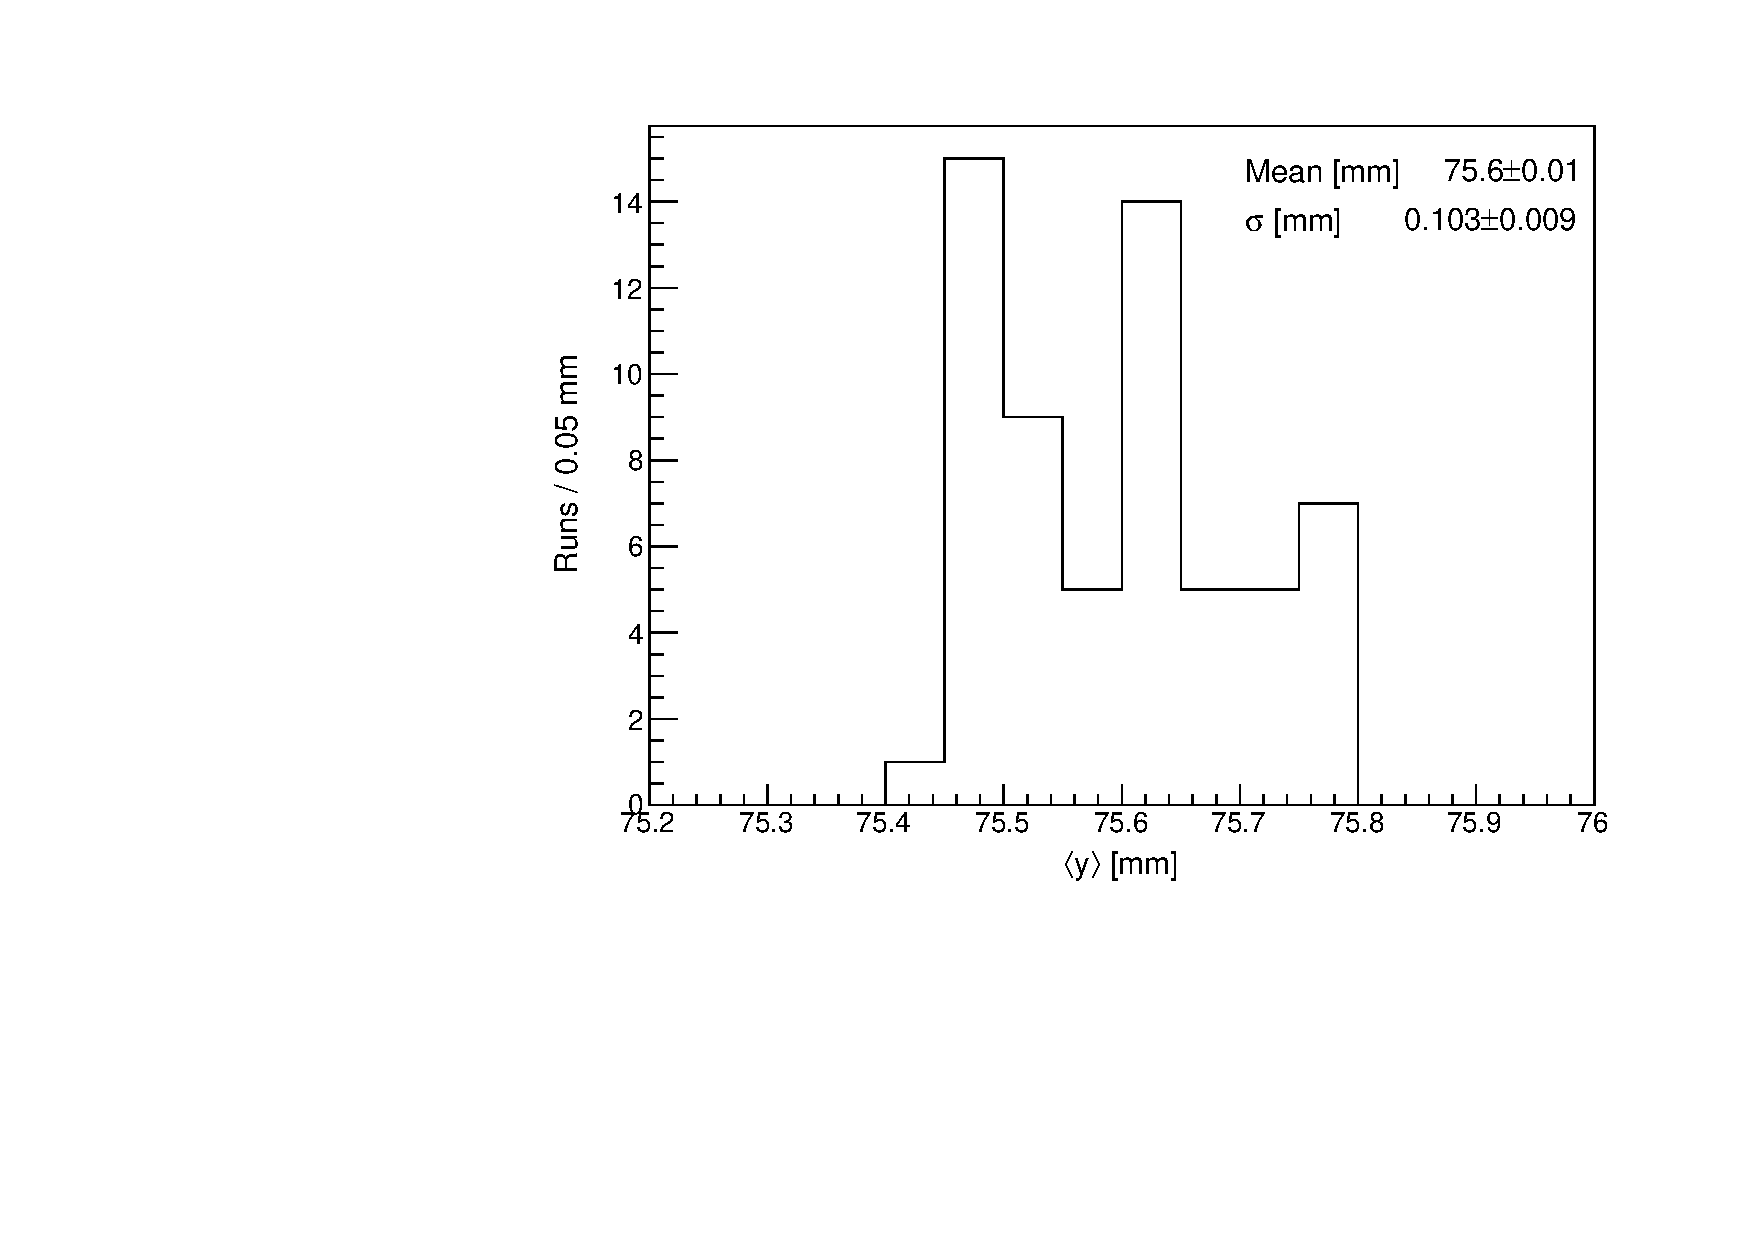
\includegraphics[trim={0 0 0 0},clip,width=0.49\textwidth]{Images/Chapter4/h_yRunAvg_gm2pro_daq_full_run1_60h_5039A_GLdocDB16021-v2_15921_15991.pdf}\label{subfig:hDeltaY60h} }
\caption{Assessment of the systematic uncertainties $\delta_{\text{align}}$ and $\delta_{\text{drift}}$ in Run-1a, showing: (a) the difference in measured $\langle y \rangle$ between adjacent pairs of the twenty four calorimeters, where $n=1$ represents the pair $\langle y_{1} \rangle - \langle y_{2} \rangle$; (b) the distribution of those differences compared to Run-4, the width of which was taken as $\delta_{\text{align}}$; (c) the distribution of $\langle y \rangle$, where again, the width was taken as the uncertainty $\delta_{\text{drift}}$.}
\label{fig:BrSystPlots}
\end{figure}  


\afterpage{
\begin{table}[]
\centering
\begin{tabular}{cccc}
\hline
\hline
Dataset & $\delta_{\text{stat}}$ [mm] & $\delta_{\text{align}}$ [mm] & $\delta_{\text{drift}}$ [mm] \\
\hline
1a & $7.28\times10^{-4}$ & 0.348 & 0.103 \\
1b & $6.28\times10^{-4}$ & 0.354 & 0.109 \\
1c & $5.29\times10^{-4}$ & 0.369 & 0.0480 \\
1d & $4.12\times10^{-4}$ & 0.425 & 0.162 \\
\hdashline 
2b & $8.25\times10^{-4}$ & 0.175 & 0.0381 \\ 
2c & $4.05\times10^{-4}$ & 0.183 & 0.0631 \\
2d & $4.46\times10^{-4}$ & 0.298 & 0.0914 \\
2e & $6.75\times10^{-4}$ & 0.173 & 0.0385 \\
2f & $6.44\times10^{-4}$ & 0.173 & 0.0450 \\
2g & $1.80\times10^{-3}$ & 0.236 & 0.0600 \\
2h & $1.14\times10^{-3}$ & 0.246 & 0.0208 \\
\hdashline
3N & $4.36\times10^{-4}$ & 0.247 & 0.0316 \\ 
3O & $4.82\times10^{-4}$ & 0.269 & 0.0233 \\
\hdashline
4 (NL) & $3.37\times10^{-4}$ & 0.0235 & 0.0510 \\
\hdashline  
5 (NL) & $3.88\times10^{-4}$ & 0.171 & 0.0224 \\ 
\hline
\hline
\end{tabular}
\caption{Contributions to the uncertainty on the estimated total radial magnetic field in each datasets. Estimates in Run-4 and Run-5 were made using nearline (NL) data, and so are preliminary.}
\label{tbl:BrUncertainties}
\end{table}
%
\begin{figure}[]
\centering{}
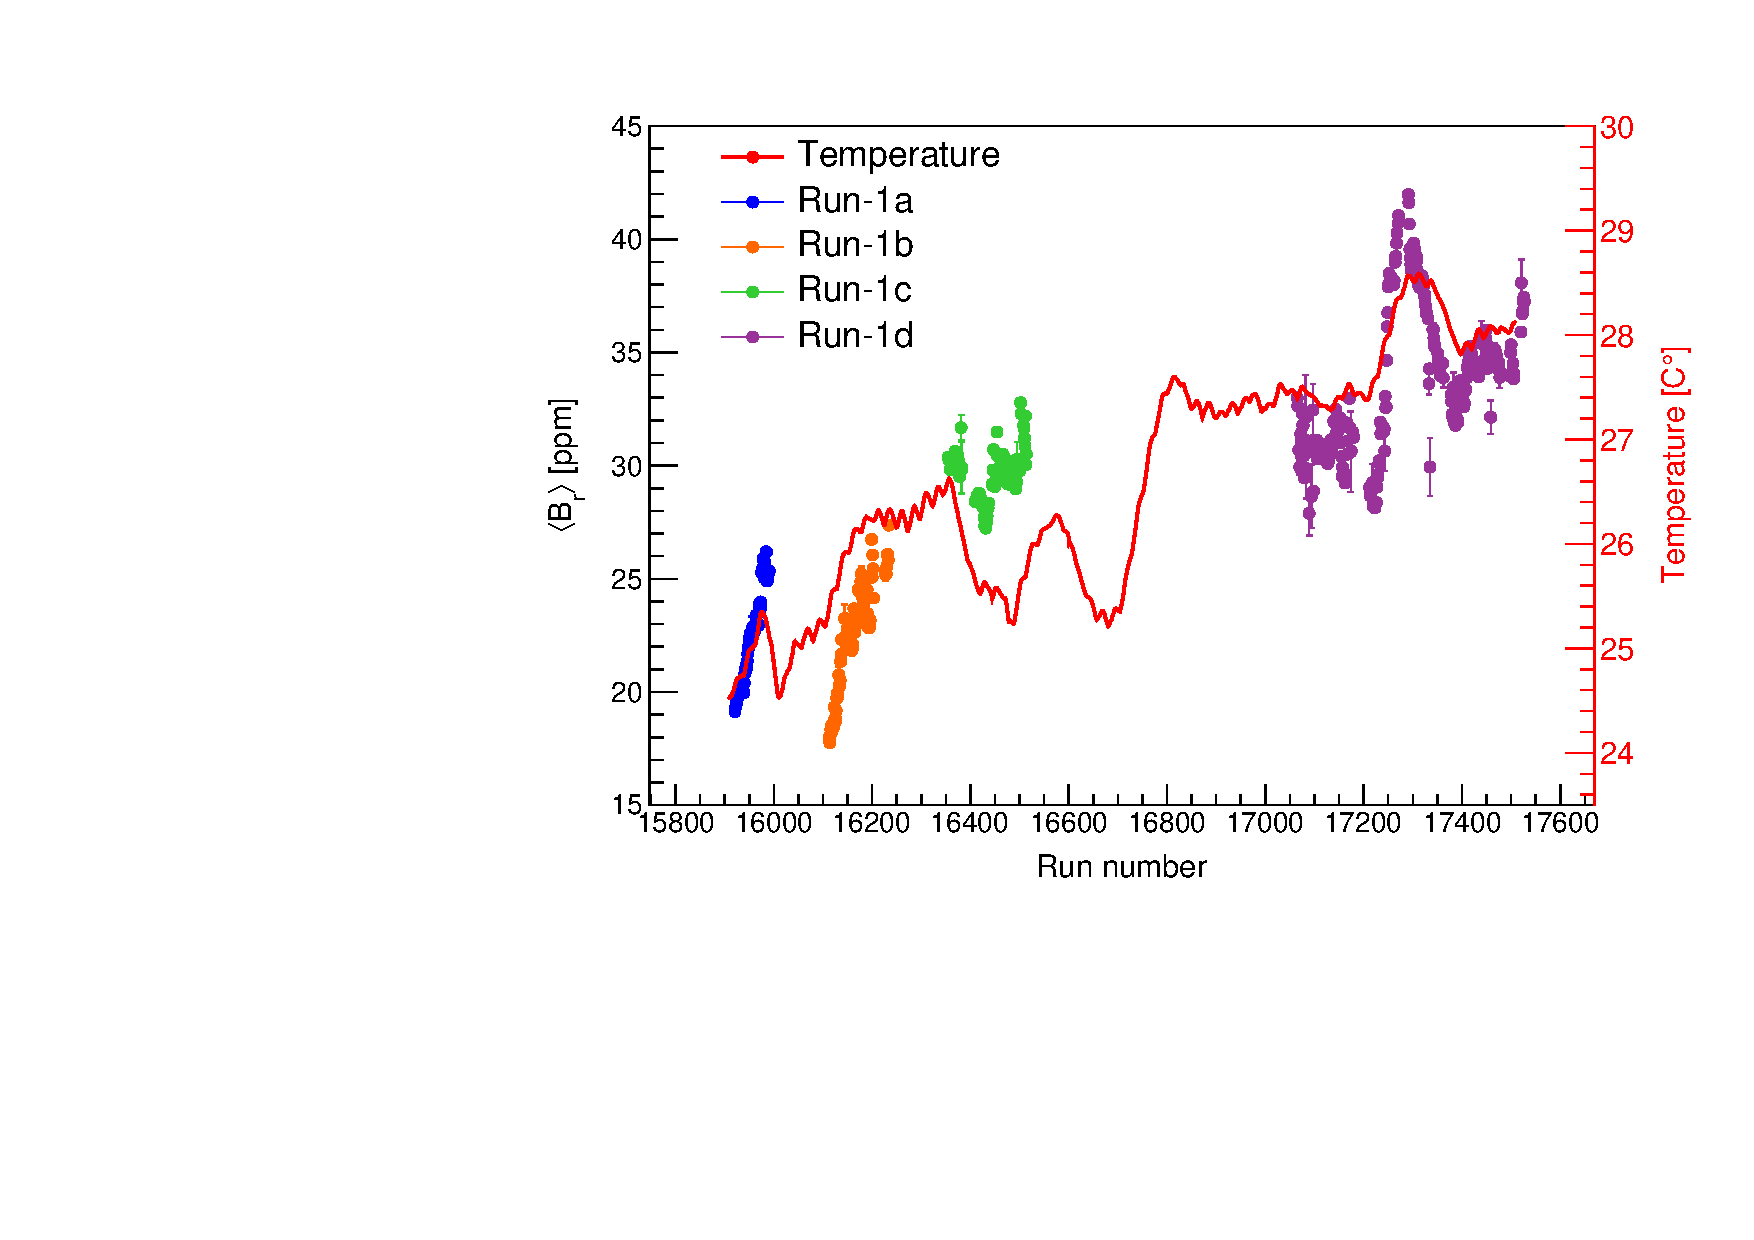
\includegraphics[trim={0 0 0 0},clip,width=0.69\textwidth]{Images/Chapter4/BrTempOverlayRun1.pdf}
\caption{The estimated $\langle B_{r} \rangle$ throughout Run-1. The observed variation appears to be correlated with the temperature as measured by a probe inside the experiment hall, which is overlaid on a secondary scale for comparison. The uncertainties associated with each data-point are purely statistical. Temperature data courtesy of D. Vasilkova \cite{HallTemp}.}
\label{fig:BrTempOverlay}
\end{figure}
% 
\clearpage
%
\begin{figure}[]
\centering{}
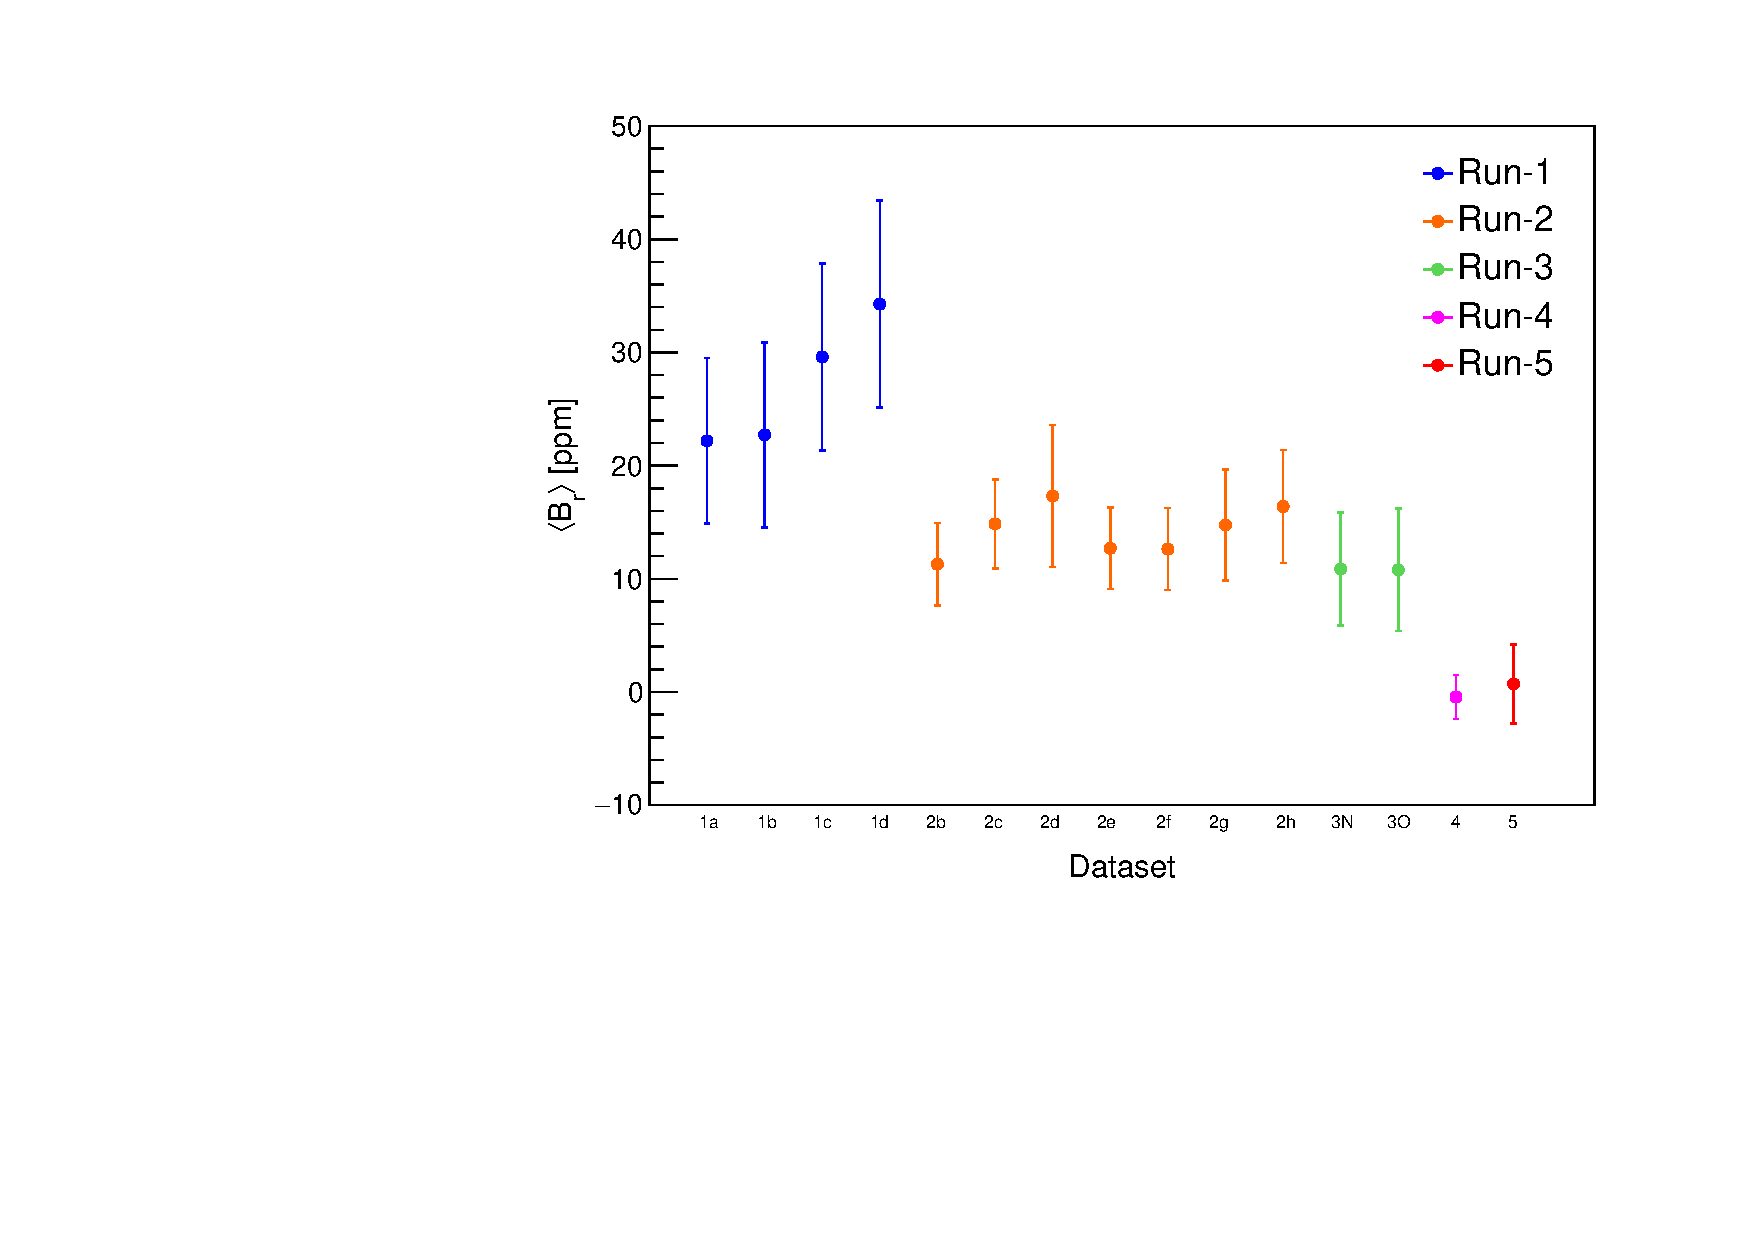
\includegraphics[trim={0 0 0 0},clip,width=0.79\textwidth]{Images/Chapter4/BrVsDS2_empiricalMethod.pdf}
\caption{Estimates for $\langle B_{r} \rangle$ in ppm for various E989 datasets. The estimates for Run-4 and Run-5 are preliminary.}
\label{fig:BrVsDS}
\end{figure}   
%
\begin{table}[]
\centering
\begin{tabular}{ccc}
\hline
\hline
Dataset & $\langle B_{r} \rangle$ [ppm] & Equivalent $d_{\mu}$ [$\times10^{-20}$ $e\cdot$cm] \\ 
\hline
1a & $22\pm7$ & $7\pm2$ \\ 
1b & $23\pm8$ & $7\pm3$ \\
1c & $30\pm8$ & $9\pm3$ \\
1d & $34\pm9$ & $10\pm3$ \\ 
\hdashline 
2b & $11\pm4$ & $4\pm1$ \\
2c & $15\pm4$ & $5\pm1$ \\
2d & $17\pm6$ & $6\pm2$ \\
2e & $13\pm4$ & $4\pm1$ \\
2f & $13\pm4$ & $4\pm1$ \\
2g & $15\pm5$ & $5\pm2$ \\
2h & $16\pm5$ & $5\pm2$ \\
\hdashline
3N & $11\pm5$ & $3\pm2$ \\
3O & $11\pm5$ & $3\pm2$ \\
\hdashline
4 (NL) & $-0.4\pm2.0$ & $-0.1\pm0.6$ \\
\hdashline
5 (NL) & $0.7\pm3.5$ & $0.2\pm1.1$ \\
\hline
\hline
\end{tabular}
\caption{Estimates for $\langle B_{r} \rangle$ in ppm, as well as the equivalent fake EDM signal in $e\cdot$cm, for various E989 datasets. The uncertainties for Run-1 are within the 10 ppm target stated in Section \ref{sec:BrPrecision}.}
\label{tbl:BrResults}
\end{table}
\clearpage
}

The systematic contributions from calorimeter misalignment and field drift, $\delta_{\text{align}}$ and $\delta_{\text{drift}}$, were then estimated (following the method detailed in Section \ref{subsection:ExtrapolatingTheRadialField}). An example of the relative misalignment per calorimeter in Run-1a compared to Run-4 is shown in Figure \ref{subfig:grComp}, where the width of the distribution in Figure \ref{subfig:hDiff} was taken as $\delta_{\text{align}}$ for that dataset. An example distribution of $\langle y \rangle$ for Run-1a, the width of which was taken as $\delta_{\text{drift}}$ for that dataset, is shown in Figure \ref{subfig:hDeltaY60h}. These systematic uncertainties are reported, alongside the statistical contribution, $\delta_{\text{stat}}$, for various E989 dataset in Table \ref{tbl:BrUncertainties}. The contribution from calorimeter misalignment dominates. 

For the purposes of illustration, the estimated $\langle B_{r} \rangle$ per run is presented for Run-1 in Figure \ref{fig:BrTempOverlay}, where the uncertainty per run is taken as purely statistical. Significant variation may be seen both within and between datasets, which appears to be correlated with the temperature as measured by a probe inside the experiment hall. The cause of this correlation is thought to arise from the expansion and contraction of the C-shaped yoke with varying hall temperature. Since Run-1, the addition of thermal insulation around the magnet, as well as improvements to the climate control inside the experiment hall, appear to have minimised this effect. 

Finally, the results for $\langle B_{r} \rangle$ are presented in Figure \ref{fig:BrVsDS} and Table \ref{tbl:BrResults}, which includes to the total uncertainty $\delta \langle B_{r} \rangle$. The equivalent laboratory frame precession plane tilt angle is also given in units of $e\cdot$cm, which is obtained by first taking $\langle B_{r} \rangle$ in units of ppm to be equivalent to \SI{}{\micro\radian} by the small angle approximation, so that the laboratory frame tilt angle is given by
%
\begin{equation}
  \delta = \frac{B_{r}}{B_{y}},
\end{equation}
% 
and calculating the equivalent fake muon EDM signal by Equation \ref{eqn:EDMFromAngle}. These values will eventually be subtracted from the measured muon EDM signal. 

\section{Summary and outlook}

The average background radial field, $\langle B_{r}^{b} \rangle$, was measured in E989 Run-4 by use of a novel ESQ/SCC scan-based method. Two measurements were performed. The first was a preliminary measurement performed on the \nth{8}--\nth{9} of December 2020, during a period with low beam intensity (10\% of Run-3), where $\langle B_{r}^{b} \rangle$ was measured to be $15\pm1$ ppm. Following this result, SCC currents adjusted were to cancel the background, so that the total field, $\langle B_{r} \rangle$, was set to zero. A second measurement was then performed on the \nth{30} December 2020 with nominal beam intensity, whereupon $\langle B_{r}^{b} \rangle$ was found to $-0.4\pm0.6$ ppm, which is consistent with zero. The target uncertainty for this measurement, based on the statistically limited case for a muon EDM search using the E989 integrated dataset, was $\leq$1 ppm, which is achieved by this measurement. This result was then extrapolated, based on the change in ring average vertical beam position, to estimate $\langle B_{r} \rangle$ for all available E989 datasets. These estimates are reported in Figure \ref{fig:BrVsDS} and Table \ref{tbl:BrResults}. In the case of the Run-1 datasets, the uncertainties fall within the target of $\leq$10 ppm (for 100 million high quality tracks), meaning that the search for a muon EDM in Run-1 is not limited by the radial field systematic.

The ESQ/SCC scan-based method has the significant advantage over measurements which involve the use of additional hardware, such as hall probes, in that it does not require any physical modifications to the experiment, and may be accomplished in a relatively short period of beam-time. Since the time of writing, the methods described in this chapter have been used by fellow E989 collaborators to conduct a measurement of $\langle B_{r}^{b} \rangle$ in Run-5, and produce estimates of the radial field in further E989 datasets as they are produced.